% Options for packages loaded elsewhere
\PassOptionsToPackage{unicode}{hyperref}
\PassOptionsToPackage{hyphens}{url}
%
\documentclass[
]{article}
\usepackage{amsmath,amssymb}
\usepackage{lmodern}
\usepackage{iftex}
\ifPDFTeX
  \usepackage[T1]{fontenc}
  \usepackage[utf8]{inputenc}
  \usepackage{textcomp} % provide euro and other symbols
\else % if luatex or xetex
  \usepackage{unicode-math}
  \defaultfontfeatures{Scale=MatchLowercase}
  \defaultfontfeatures[\rmfamily]{Ligatures=TeX,Scale=1}
\fi
% Use upquote if available, for straight quotes in verbatim environments
\IfFileExists{upquote.sty}{\usepackage{upquote}}{}
\IfFileExists{microtype.sty}{% use microtype if available
  \usepackage[]{microtype}
  \UseMicrotypeSet[protrusion]{basicmath} % disable protrusion for tt fonts
}{}
\makeatletter
\@ifundefined{KOMAClassName}{% if non-KOMA class
  \IfFileExists{parskip.sty}{%
    \usepackage{parskip}
  }{% else
    \setlength{\parindent}{0pt}
    \setlength{\parskip}{6pt plus 2pt minus 1pt}}
}{% if KOMA class
  \KOMAoptions{parskip=half}}
\makeatother
\usepackage{xcolor}
\IfFileExists{xurl.sty}{\usepackage{xurl}}{} % add URL line breaks if available
\IfFileExists{bookmark.sty}{\usepackage{bookmark}}{\usepackage{hyperref}}
\hypersetup{
  pdftitle={PCCA Survey 2022},
  pdfauthor={Don Lim},
  hidelinks,
  pdfcreator={LaTeX via pandoc}}
\urlstyle{same} % disable monospaced font for URLs
\usepackage[margin=1in]{geometry}
\usepackage{color}
\usepackage{fancyvrb}
\newcommand{\VerbBar}{|}
\newcommand{\VERB}{\Verb[commandchars=\\\{\}]}
\DefineVerbatimEnvironment{Highlighting}{Verbatim}{commandchars=\\\{\}}
% Add ',fontsize=\small' for more characters per line
\usepackage{framed}
\definecolor{shadecolor}{RGB}{248,248,248}
\newenvironment{Shaded}{\begin{snugshade}}{\end{snugshade}}
\newcommand{\AlertTok}[1]{\textcolor[rgb]{0.94,0.16,0.16}{#1}}
\newcommand{\AnnotationTok}[1]{\textcolor[rgb]{0.56,0.35,0.01}{\textbf{\textit{#1}}}}
\newcommand{\AttributeTok}[1]{\textcolor[rgb]{0.77,0.63,0.00}{#1}}
\newcommand{\BaseNTok}[1]{\textcolor[rgb]{0.00,0.00,0.81}{#1}}
\newcommand{\BuiltInTok}[1]{#1}
\newcommand{\CharTok}[1]{\textcolor[rgb]{0.31,0.60,0.02}{#1}}
\newcommand{\CommentTok}[1]{\textcolor[rgb]{0.56,0.35,0.01}{\textit{#1}}}
\newcommand{\CommentVarTok}[1]{\textcolor[rgb]{0.56,0.35,0.01}{\textbf{\textit{#1}}}}
\newcommand{\ConstantTok}[1]{\textcolor[rgb]{0.00,0.00,0.00}{#1}}
\newcommand{\ControlFlowTok}[1]{\textcolor[rgb]{0.13,0.29,0.53}{\textbf{#1}}}
\newcommand{\DataTypeTok}[1]{\textcolor[rgb]{0.13,0.29,0.53}{#1}}
\newcommand{\DecValTok}[1]{\textcolor[rgb]{0.00,0.00,0.81}{#1}}
\newcommand{\DocumentationTok}[1]{\textcolor[rgb]{0.56,0.35,0.01}{\textbf{\textit{#1}}}}
\newcommand{\ErrorTok}[1]{\textcolor[rgb]{0.64,0.00,0.00}{\textbf{#1}}}
\newcommand{\ExtensionTok}[1]{#1}
\newcommand{\FloatTok}[1]{\textcolor[rgb]{0.00,0.00,0.81}{#1}}
\newcommand{\FunctionTok}[1]{\textcolor[rgb]{0.00,0.00,0.00}{#1}}
\newcommand{\ImportTok}[1]{#1}
\newcommand{\InformationTok}[1]{\textcolor[rgb]{0.56,0.35,0.01}{\textbf{\textit{#1}}}}
\newcommand{\KeywordTok}[1]{\textcolor[rgb]{0.13,0.29,0.53}{\textbf{#1}}}
\newcommand{\NormalTok}[1]{#1}
\newcommand{\OperatorTok}[1]{\textcolor[rgb]{0.81,0.36,0.00}{\textbf{#1}}}
\newcommand{\OtherTok}[1]{\textcolor[rgb]{0.56,0.35,0.01}{#1}}
\newcommand{\PreprocessorTok}[1]{\textcolor[rgb]{0.56,0.35,0.01}{\textit{#1}}}
\newcommand{\RegionMarkerTok}[1]{#1}
\newcommand{\SpecialCharTok}[1]{\textcolor[rgb]{0.00,0.00,0.00}{#1}}
\newcommand{\SpecialStringTok}[1]{\textcolor[rgb]{0.31,0.60,0.02}{#1}}
\newcommand{\StringTok}[1]{\textcolor[rgb]{0.31,0.60,0.02}{#1}}
\newcommand{\VariableTok}[1]{\textcolor[rgb]{0.00,0.00,0.00}{#1}}
\newcommand{\VerbatimStringTok}[1]{\textcolor[rgb]{0.31,0.60,0.02}{#1}}
\newcommand{\WarningTok}[1]{\textcolor[rgb]{0.56,0.35,0.01}{\textbf{\textit{#1}}}}
\usepackage{graphicx}
\makeatletter
\def\maxwidth{\ifdim\Gin@nat@width>\linewidth\linewidth\else\Gin@nat@width\fi}
\def\maxheight{\ifdim\Gin@nat@height>\textheight\textheight\else\Gin@nat@height\fi}
\makeatother
% Scale images if necessary, so that they will not overflow the page
% margins by default, and it is still possible to overwrite the defaults
% using explicit options in \includegraphics[width, height, ...]{}
\setkeys{Gin}{width=\maxwidth,height=\maxheight,keepaspectratio}
% Set default figure placement to htbp
\makeatletter
\def\fps@figure{htbp}
\makeatother
\setlength{\emergencystretch}{3em} % prevent overfull lines
\providecommand{\tightlist}{%
  \setlength{\itemsep}{0pt}\setlength{\parskip}{0pt}}
\setcounter{secnumdepth}{-\maxdimen} % remove section numbering
\usepackage{booktabs}
\usepackage{longtable}
\usepackage{array}
\usepackage{multirow}
\usepackage{wrapfig}
\usepackage{float}
\usepackage{colortbl}
\usepackage{pdflscape}
\usepackage{tabu}
\usepackage{threeparttable}
\usepackage{threeparttablex}
\usepackage[normalem]{ulem}
\usepackage{makecell}
\usepackage{xcolor}
\ifLuaTeX
  \usepackage{selnolig}  % disable illegal ligatures
\fi

\title{PCCA Survey 2022}
\author{Don Lim}
\date{4/6/2022}

\begin{document}
\maketitle

{
\setcounter{tocdepth}{2}
\tableofcontents
}
\begin{Shaded}
\begin{Highlighting}[]
\FunctionTok{library}\NormalTok{(readxl)}
\FunctionTok{library}\NormalTok{(tidyverse)}
\FunctionTok{library}\NormalTok{(dplyr)}
\FunctionTok{library}\NormalTok{(ggplot2)}
\FunctionTok{library}\NormalTok{(scales)}
\FunctionTok{library}\NormalTok{(estimatr)}
\FunctionTok{library}\NormalTok{(stargazer)}
\FunctionTok{library}\NormalTok{(pastecs)}
\FunctionTok{library}\NormalTok{(reshape2)}

\FunctionTok{library}\NormalTok{(ggpubr)}
\FunctionTok{library}\NormalTok{(rstatix)}
\FunctionTok{library}\NormalTok{(vtable)}
\end{Highlighting}
\end{Shaded}

\hypertarget{data-cleanup}{%
\section{Data cleanup}\label{data-cleanup}}

Imports data and removes redundant first row

\begin{Shaded}
\begin{Highlighting}[]
\NormalTok{survey }\OtherTok{\textless{}{-}} \FunctionTok{read\_excel}\NormalTok{(}\StringTok{"SoGoSurvey\_PCCA Grower{-}Owner Survey 3{-}25{-}22.xls"}\NormalTok{,}
    \AttributeTok{col\_types =} \FunctionTok{c}\NormalTok{(}\StringTok{"skip"}\NormalTok{, }\StringTok{"text"}\NormalTok{, }\StringTok{"text"}\NormalTok{, }\StringTok{"text"}\NormalTok{, }\StringTok{"text"}\NormalTok{, }\StringTok{"text"}\NormalTok{,}
        \StringTok{"text"}\NormalTok{, }\StringTok{"text"}\NormalTok{, }\StringTok{"text"}\NormalTok{, }\StringTok{"text"}\NormalTok{, }\StringTok{"text"}\NormalTok{, }\StringTok{"text"}\NormalTok{, }\StringTok{"text"}\NormalTok{,}
        \StringTok{"text"}\NormalTok{, }\StringTok{"text"}\NormalTok{, }\StringTok{"text"}\NormalTok{, }\StringTok{"text"}\NormalTok{, }\StringTok{"text"}\NormalTok{, }\StringTok{"text"}\NormalTok{, }\StringTok{"text"}\NormalTok{,}
        \StringTok{"text"}\NormalTok{, }\StringTok{"text"}\NormalTok{, }\StringTok{"text"}\NormalTok{, }\StringTok{"text"}\NormalTok{, }\StringTok{"text"}\NormalTok{, }\StringTok{"text"}\NormalTok{, }\StringTok{"text"}\NormalTok{,}
        \StringTok{"text"}\NormalTok{, }\StringTok{"text"}\NormalTok{, }\StringTok{"text"}\NormalTok{, }\StringTok{"text"}\NormalTok{, }\StringTok{"text"}\NormalTok{, }\StringTok{"text"}\NormalTok{, }\StringTok{"text"}\NormalTok{,}
        \StringTok{"text"}\NormalTok{, }\StringTok{"text"}\NormalTok{, }\StringTok{"text"}\NormalTok{, }\StringTok{"text"}\NormalTok{, }\StringTok{"text"}\NormalTok{, }\StringTok{"text"}\NormalTok{, }\StringTok{"text"}\NormalTok{,}
        \StringTok{"text"}\NormalTok{, }\StringTok{"text"}\NormalTok{, }\StringTok{"text"}\NormalTok{, }\StringTok{"text"}\NormalTok{, }\StringTok{"text"}\NormalTok{, }\StringTok{"text"}\NormalTok{, }\StringTok{"text"}\NormalTok{,}
        \StringTok{"text"}\NormalTok{, }\StringTok{"text"}\NormalTok{, }\StringTok{"text"}\NormalTok{, }\StringTok{"text"}\NormalTok{, }\StringTok{"text"}\NormalTok{, }\StringTok{"text"}\NormalTok{, }\StringTok{"text"}\NormalTok{,}
        \StringTok{"text"}\NormalTok{, }\StringTok{"text"}\NormalTok{, }\StringTok{"text"}\NormalTok{, }\StringTok{"text"}\NormalTok{, }\StringTok{"text"}\NormalTok{, }\StringTok{"text"}\NormalTok{, }\StringTok{"text"}\NormalTok{,}
        \StringTok{"text"}\NormalTok{, }\StringTok{"text"}\NormalTok{, }\StringTok{"text"}\NormalTok{, }\StringTok{"text"}\NormalTok{, }\StringTok{"text"}\NormalTok{, }\StringTok{"text"}\NormalTok{, }\StringTok{"text"}\NormalTok{,}
        \StringTok{"text"}\NormalTok{, }\StringTok{"text"}\NormalTok{, }\StringTok{"text"}\NormalTok{, }\StringTok{"text"}\NormalTok{, }\StringTok{"text"}\NormalTok{, }\StringTok{"text"}\NormalTok{, }\StringTok{"text"}\NormalTok{,}
        \StringTok{"text"}\NormalTok{, }\StringTok{"text"}\NormalTok{, }\StringTok{"text"}\NormalTok{, }\StringTok{"text"}\NormalTok{, }\StringTok{"text"}\NormalTok{, }\StringTok{"text"}\NormalTok{, }\StringTok{"text"}\NormalTok{))}

\NormalTok{survey }\OtherTok{\textless{}{-}}\NormalTok{ survey[}\SpecialCharTok{{-}}\FunctionTok{c}\NormalTok{(}\DecValTok{1}\NormalTok{), ]}
\NormalTok{survey }\OtherTok{\textless{}{-}}\NormalTok{ survey[}\SpecialCharTok{{-}}\FunctionTok{c}\NormalTok{(}\DecValTok{355}\SpecialCharTok{:}\DecValTok{362}\NormalTok{), ]}
\end{Highlighting}
\end{Shaded}

Rename columns

\begin{Shaded}
\begin{Highlighting}[]
\FunctionTok{names}\NormalTok{(survey) }\OtherTok{\textless{}{-}} \FunctionTok{c}\NormalTok{(}\StringTok{"number"}\NormalTok{, }\StringTok{"status"}\NormalTok{, }\StringTok{"gathering information"}\NormalTok{,}
    \StringTok{"social media"}\NormalTok{, }\StringTok{"traditional media"}\NormalTok{, }\StringTok{"interpersonal communication"}\NormalTok{,}
    \StringTok{"industry organization"}\NormalTok{, }\StringTok{"my cooperative"}\NormalTok{, }\StringTok{"other"}\NormalTok{, }\StringTok{"new media"}\NormalTok{,}
    \StringTok{"facebook"}\NormalTok{, }\StringTok{"twitter"}\NormalTok{, }\StringTok{"instagram"}\NormalTok{, }\StringTok{"youtube"}\NormalTok{, }\StringTok{"snapchat"}\NormalTok{,}
    \StringTok{"tiktok"}\NormalTok{, }\StringTok{"other2"}\NormalTok{, }\StringTok{"podcast or radio"}\NormalTok{, }\StringTok{"podcast list"}\NormalTok{, }\StringTok{"satisfaction"}\NormalTok{,}
    \StringTok{"market information"}\NormalTok{, }\StringTok{"crop information"}\NormalTok{, }\StringTok{"industry news"}\NormalTok{,}
    \StringTok{"farm operation"}\NormalTok{, }\StringTok{"other3"}\NormalTok{, }\StringTok{"website"}\NormalTok{, }\StringTok{"email"}\NormalTok{, }\StringTok{"member access"}\NormalTok{,}
    \StringTok{"mypcca"}\NormalTok{, }\StringTok{"text"}\NormalTok{, }\StringTok{"social media2"}\NormalTok{, }\StringTok{"print"}\NormalTok{, }\StringTok{"local coop"}\NormalTok{,}
    \StringTok{"other4"}\NormalTok{, }\StringTok{"area pcca does best"}\NormalTok{, }\StringTok{"mypcca app"}\NormalTok{, }\StringTok{"social media3"}\NormalTok{,}
    \StringTok{"email2"}\NormalTok{, }\StringTok{"text2"}\NormalTok{, }\StringTok{"printed"}\NormalTok{, }\StringTok{"other5"}\NormalTok{, }\StringTok{"communication improvements"}\NormalTok{,}
    \StringTok{"topic"}\NormalTok{, }\StringTok{"accessible"}\NormalTok{, }\StringTok{"responsive"}\NormalTok{, }\StringTok{"courteous"}\NormalTok{, }\StringTok{"marketing pool"}\NormalTok{,}
    \StringTok{"the seam"}\NormalTok{, }\StringTok{"pcca direct"}\NormalTok{, }\StringTok{"forward contracting"}\NormalTok{, }\StringTok{"most used marketing method"}\NormalTok{,}
    \StringTok{"information"}\NormalTok{, }\StringTok{"change"}\NormalTok{, }\StringTok{"influence"}\NormalTok{, }\StringTok{"best performance"}\NormalTok{,}
    \StringTok{"minimize risk"}\NormalTok{, }\StringTok{"control"}\NormalTok{, }\StringTok{"reliability"}\NormalTok{, }\StringTok{"price information"}\NormalTok{,}
    \StringTok{"why member"}\NormalTok{, }\StringTok{"opportunities"}\NormalTok{, }\StringTok{"how"}\NormalTok{, }\StringTok{"open and voluntary"}\NormalTok{,}
    \StringTok{"member control"}\NormalTok{, }\StringTok{"economic participation"}\NormalTok{, }\StringTok{"autonomy"}\NormalTok{, }\StringTok{"education"}\NormalTok{,}
    \StringTok{"cooperation"}\NormalTok{, }\StringTok{"community"}\NormalTok{, }\StringTok{"coop vs noncoop"}\NormalTok{, }\StringTok{"knowledge of coop"}\NormalTok{,}
    \StringTok{"coop meetings"}\NormalTok{, }\StringTok{"up to date"}\NormalTok{, }\StringTok{"age"}\NormalTok{, }\StringTok{"description"}\NormalTok{, }\StringTok{"active"}\NormalTok{,}
    \StringTok{"farming duration"}\NormalTok{, }\StringTok{"region"}\NormalTok{, }\StringTok{"operation"}\NormalTok{, }\StringTok{"education level"}\NormalTok{,}
    \StringTok{"membership duration"}\NormalTok{, }\StringTok{"thoughts"}\NormalTok{)}
\end{Highlighting}
\end{Shaded}

Dummy variables

Replaces 1 if true, 0 if false

\begin{Shaded}
\begin{Highlighting}[]
\NormalTok{survey }\OtherTok{\textless{}{-}} \FunctionTok{mutate\_at}\NormalTok{(survey, }\FunctionTok{c}\NormalTok{(}\StringTok{"social media"}\NormalTok{, }\StringTok{"traditional media"}\NormalTok{,}
    \StringTok{"interpersonal communication"}\NormalTok{, }\StringTok{"industry organization"}\NormalTok{, }\StringTok{"my cooperative"}\NormalTok{,}
    \StringTok{"facebook"}\NormalTok{, }\StringTok{"twitter"}\NormalTok{, }\StringTok{"instagram"}\NormalTok{, }\StringTok{"youtube"}\NormalTok{, }\StringTok{"snapchat"}\NormalTok{,}
    \StringTok{"tiktok"}\NormalTok{, }\StringTok{"market information"}\NormalTok{, }\StringTok{"crop information"}\NormalTok{, }\StringTok{"industry news"}\NormalTok{,}
    \StringTok{"farm operation"}\NormalTok{, }\StringTok{"website"}\NormalTok{, }\StringTok{"email"}\NormalTok{, }\StringTok{"member access"}\NormalTok{, }\StringTok{"mypcca"}\NormalTok{,}
    \StringTok{"text"}\NormalTok{, }\StringTok{"social media2"}\NormalTok{, }\StringTok{"print"}\NormalTok{, }\StringTok{"local coop"}\NormalTok{, }\StringTok{"mypcca app"}\NormalTok{,}
    \StringTok{"social media3"}\NormalTok{, }\StringTok{"email2"}\NormalTok{, }\StringTok{"text2"}\NormalTok{, }\StringTok{"printed"}\NormalTok{), }\SpecialCharTok{\textasciitilde{}}\FunctionTok{replace}\NormalTok{(.,}
    \SpecialCharTok{!}\FunctionTok{is.na}\NormalTok{(.), }\DecValTok{1}\NormalTok{))}

\NormalTok{survey }\OtherTok{\textless{}{-}} \FunctionTok{mutate\_at}\NormalTok{(survey, }\FunctionTok{c}\NormalTok{(}\StringTok{"social media"}\NormalTok{, }\StringTok{"traditional media"}\NormalTok{,}
    \StringTok{"interpersonal communication"}\NormalTok{, }\StringTok{"industry organization"}\NormalTok{, }\StringTok{"my cooperative"}\NormalTok{,}
    \StringTok{"facebook"}\NormalTok{, }\StringTok{"twitter"}\NormalTok{, }\StringTok{"instagram"}\NormalTok{, }\StringTok{"youtube"}\NormalTok{, }\StringTok{"snapchat"}\NormalTok{,}
    \StringTok{"tiktok"}\NormalTok{, }\StringTok{"market information"}\NormalTok{, }\StringTok{"crop information"}\NormalTok{, }\StringTok{"industry news"}\NormalTok{,}
    \StringTok{"farm operation"}\NormalTok{, }\StringTok{"website"}\NormalTok{, }\StringTok{"email"}\NormalTok{, }\StringTok{"member access"}\NormalTok{, }\StringTok{"mypcca"}\NormalTok{,}
    \StringTok{"text"}\NormalTok{, }\StringTok{"social media2"}\NormalTok{, }\StringTok{"print"}\NormalTok{, }\StringTok{"local coop"}\NormalTok{, }\StringTok{"mypcca app"}\NormalTok{,}
    \StringTok{"social media3"}\NormalTok{, }\StringTok{"email2"}\NormalTok{, }\StringTok{"text2"}\NormalTok{, }\StringTok{"printed"}\NormalTok{), }\SpecialCharTok{\textasciitilde{}}\FunctionTok{replace}\NormalTok{(.,}
    \FunctionTok{is.na}\NormalTok{(.), }\DecValTok{0}\NormalTok{))}
\end{Highlighting}
\end{Shaded}

\begin{Shaded}
\begin{Highlighting}[]
\NormalTok{survey }\OtherTok{\textless{}{-}}\NormalTok{ survey }\SpecialCharTok{\%\textgreater{}\%}
    \FunctionTok{mutate}\NormalTok{(}\FunctionTok{across}\NormalTok{(}\FunctionTok{c}\NormalTok{(}\StringTok{\textasciigrave{}}\AttributeTok{new media}\StringTok{\textasciigrave{}}\NormalTok{, }\StringTok{\textasciigrave{}}\AttributeTok{podcast or radio}\StringTok{\textasciigrave{}}\NormalTok{, opportunities,}
\NormalTok{        active), }\SpecialCharTok{\textasciitilde{}}\FunctionTok{factor}\NormalTok{(}\FunctionTok{ifelse}\NormalTok{(.x }\SpecialCharTok{==} \StringTok{"Yes"}\NormalTok{, }\DecValTok{1}\NormalTok{, }\DecValTok{0}\NormalTok{))))}
\end{Highlighting}
\end{Shaded}

Converts Likert answers to numerical values: Strongly disagree is 1,
disagree is 2, somewhat disagree is 3, somewhat agree is 4, agree is 5,
and strongly agree is 6. Also changes knowledge answers to numerical
values: no knowledge is 1, some knowledge is 2, and extensive knowledge
is 3.

\begin{Shaded}
\begin{Highlighting}[]
\NormalTok{survey }\OtherTok{\textless{}{-}} \FunctionTok{mutate\_at}\NormalTok{(survey, }\FunctionTok{c}\NormalTok{(}\StringTok{"accessible"}\NormalTok{, }\StringTok{"responsive"}\NormalTok{, }\StringTok{"courteous"}\NormalTok{,}
    \StringTok{"minimize risk"}\NormalTok{, }\StringTok{"control"}\NormalTok{, }\StringTok{"reliability"}\NormalTok{, }\StringTok{"price information"}\NormalTok{),}
    \FunctionTok{funs}\NormalTok{(}\FunctionTok{recode}\NormalTok{(., }\StringTok{\textasciigrave{}}\AttributeTok{Strongly Disagree}\StringTok{\textasciigrave{}} \OtherTok{=} \DecValTok{1}\NormalTok{, }\AttributeTok{Disagree =} \DecValTok{2}\NormalTok{, }\StringTok{\textasciigrave{}}\AttributeTok{Somewhat Disagree}\StringTok{\textasciigrave{}} \OtherTok{=} \DecValTok{3}\NormalTok{,}
        \StringTok{\textasciigrave{}}\AttributeTok{Somewhat Agree}\StringTok{\textasciigrave{}} \OtherTok{=} \DecValTok{4}\NormalTok{, }\AttributeTok{Agree =} \DecValTok{5}\NormalTok{, }\StringTok{\textasciigrave{}}\AttributeTok{Strongly Agree}\StringTok{\textasciigrave{}} \OtherTok{=} \DecValTok{6}\NormalTok{)))}

\NormalTok{survey }\OtherTok{\textless{}{-}} \FunctionTok{mutate\_at}\NormalTok{(survey, }\FunctionTok{c}\NormalTok{(}\StringTok{"marketing pool"}\NormalTok{, }\StringTok{"the seam"}\NormalTok{, }\StringTok{"pcca direct"}\NormalTok{,}
    \StringTok{"forward contracting"}\NormalTok{), }\FunctionTok{funs}\NormalTok{(}\FunctionTok{recode}\NormalTok{(., }\StringTok{\textasciigrave{}}\AttributeTok{No Knowledge}\StringTok{\textasciigrave{}} \OtherTok{=} \DecValTok{1}\NormalTok{,}
    \StringTok{\textasciigrave{}}\AttributeTok{Some Knowledge}\StringTok{\textasciigrave{}} \OtherTok{=} \DecValTok{2}\NormalTok{, }\StringTok{\textasciigrave{}}\AttributeTok{Extensive Knowledge}\StringTok{\textasciigrave{}} \OtherTok{=} \DecValTok{3}\NormalTok{)))}
\end{Highlighting}
\end{Shaded}

The following code converts character columns into numeric

\begin{Shaded}
\begin{Highlighting}[]
\NormalTok{cols.num }\OtherTok{\textless{}{-}} \FunctionTok{c}\NormalTok{(}\StringTok{"number"}\NormalTok{, }\StringTok{"social media"}\NormalTok{, }\StringTok{"traditional media"}\NormalTok{,}
    \StringTok{"interpersonal communication"}\NormalTok{, }\StringTok{"industry organization"}\NormalTok{, }\StringTok{"my cooperative"}\NormalTok{,}
    \StringTok{"new media"}\NormalTok{, }\StringTok{"facebook"}\NormalTok{, }\StringTok{"twitter"}\NormalTok{, }\StringTok{"instagram"}\NormalTok{, }\StringTok{"youtube"}\NormalTok{,}
    \StringTok{"snapchat"}\NormalTok{, }\StringTok{"tiktok"}\NormalTok{, }\StringTok{"podcast or radio"}\NormalTok{, }\StringTok{"satisfaction"}\NormalTok{,}
    \StringTok{"market information"}\NormalTok{, }\StringTok{"crop information"}\NormalTok{, }\StringTok{"industry news"}\NormalTok{,}
    \StringTok{"farm operation"}\NormalTok{, }\StringTok{"website"}\NormalTok{, }\StringTok{"email"}\NormalTok{, }\StringTok{"member access"}\NormalTok{, }\StringTok{"mypcca"}\NormalTok{,}
    \StringTok{"text"}\NormalTok{, }\StringTok{"social media2"}\NormalTok{, }\StringTok{"print"}\NormalTok{, }\StringTok{"local coop"}\NormalTok{, }\StringTok{"mypcca app"}\NormalTok{,}
    \StringTok{"social media3"}\NormalTok{, }\StringTok{"email2"}\NormalTok{, }\StringTok{"text2"}\NormalTok{, }\StringTok{"printed"}\NormalTok{, }\StringTok{"accessible"}\NormalTok{,}
    \StringTok{"responsive"}\NormalTok{, }\StringTok{"courteous"}\NormalTok{, }\StringTok{"marketing pool"}\NormalTok{, }\StringTok{"the seam"}\NormalTok{,}
    \StringTok{"pcca direct"}\NormalTok{, }\StringTok{"forward contracting"}\NormalTok{, }\StringTok{"minimize risk"}\NormalTok{, }\StringTok{"control"}\NormalTok{,}
    \StringTok{"reliability"}\NormalTok{, }\StringTok{"price information"}\NormalTok{, }\StringTok{"opportunities"}\NormalTok{, }\StringTok{"open and voluntary"}\NormalTok{,}
    \StringTok{"member control"}\NormalTok{, }\StringTok{"economic participation"}\NormalTok{, }\StringTok{"autonomy"}\NormalTok{, }\StringTok{"education"}\NormalTok{,}
    \StringTok{"cooperation"}\NormalTok{, }\StringTok{"community"}\NormalTok{, }\StringTok{"coop vs noncoop"}\NormalTok{, }\StringTok{"knowledge of coop"}\NormalTok{)}

\NormalTok{survey[cols.num] }\OtherTok{\textless{}{-}} \FunctionTok{sapply}\NormalTok{(survey[cols.num], as.numeric)}
\end{Highlighting}
\end{Shaded}

\hypertarget{data-summary}{%
\subsection{Data summary}\label{data-summary}}

\begin{Shaded}
\begin{Highlighting}[]
\FunctionTok{stat.desc}\NormalTok{(survey[cols.num])}
\end{Highlighting}
\end{Shaded}

\begin{verbatim}
##                    number social media traditional media
## nbr.val      3.540000e+02 354.00000000      354.00000000
## nbr.null     0.000000e+00 258.00000000      185.00000000
## nbr.na       0.000000e+00   0.00000000        0.00000000
## min          1.000000e+00   0.00000000        0.00000000
## max          3.540000e+02   1.00000000        1.00000000
## range        3.530000e+02   1.00000000        1.00000000
## sum          6.283500e+04  96.00000000      169.00000000
## median       1.775000e+02   0.00000000        0.00000000
## mean         1.775000e+02   0.27118644        0.47740113
## SE.mean      5.439056e+00   0.02366219        0.02658512
## CI.mean.0.95 1.069703e+01   0.04653659        0.05228514
## var          1.047250e+04   0.19820425        0.25019606
## std.dev      1.023352e+02   0.44520136        0.50019602
## coef.var     5.765365e-01   1.64168003        1.04774788
##              interpersonal communication industry organization my cooperative
## nbr.val                     354.00000000          354.00000000   354.00000000
## nbr.null                    157.00000000          175.00000000   159.00000000
## nbr.na                        0.00000000            0.00000000     0.00000000
## min                           0.00000000            0.00000000     0.00000000
## max                           1.00000000            1.00000000     1.00000000
## range                         1.00000000            1.00000000     1.00000000
## sum                         197.00000000          179.00000000   195.00000000
## median                        1.00000000            1.00000000     1.00000000
## mean                          0.55649718            0.50564972     0.55084746
## SE.mean                       0.02644188            0.02661062     0.02647435
## CI.mean.0.95                  0.05200343            0.05233528     0.05206728
## var                           0.24750724            0.25067621     0.24811543
## std.dev                       0.49750100            0.50067575     0.49811186
## coef.var                      0.89398656            0.99016321     0.90426461
##                 new media     facebook      twitter    instagram      youtube
## nbr.val      353.00000000 354.00000000 354.00000000 354.00000000 354.00000000
## nbr.null       0.00000000 220.00000000 320.00000000 325.00000000 218.00000000
## nbr.na         1.00000000   0.00000000   0.00000000   0.00000000   0.00000000
## min            1.00000000   0.00000000   0.00000000   0.00000000   0.00000000
## max            2.00000000   1.00000000   1.00000000   1.00000000   1.00000000
## range          1.00000000   1.00000000   1.00000000   1.00000000   1.00000000
## sum          510.00000000 134.00000000  34.00000000  29.00000000 136.00000000
## median         1.00000000   0.00000000   0.00000000   0.00000000   0.00000000
## mean           1.44475921   0.37853107   0.09604520   0.08192090   0.38418079
## SE.mean        0.02648694   0.02581506   0.01568281   0.01459654   0.02588851
## CI.mean.0.95   0.05209256   0.05077066   0.03084349   0.02870713   0.05091512
## var            0.24765001   0.23591172   0.08706647   0.07542293   0.23725613
## std.dev        0.49764446   0.48570744   0.29507028   0.27463235   0.48708944
## coef.var       0.34444803   1.28313757   3.07220229   3.35240871   1.26786517
##                  snapchat       tiktok podcast or radio satisfaction
## nbr.val      354.00000000 354.00000000     353.00000000 3.430000e+02
## nbr.null     336.00000000 331.00000000       0.00000000 0.000000e+00
## nbr.na         0.00000000   0.00000000       1.00000000 1.100000e+01
## min            0.00000000   0.00000000       1.00000000 1.000000e+00
## max            1.00000000   1.00000000       2.00000000 6.000000e+00
## range          1.00000000   1.00000000       1.00000000 5.000000e+00
## sum           18.00000000  23.00000000     436.00000000 1.502000e+03
## median         0.00000000   0.00000000       1.00000000 5.000000e+00
## mean           0.05084746   0.06497175       1.23512748 4.379009e+00
## SE.mean        0.01169271   0.01311859       0.02260346 6.962938e-02
## CI.mean.0.95   0.02299614   0.02580043       0.04445481 1.369557e-01
## var            0.04839871   0.06092252       0.18035346 1.662950e+00
## std.dev        0.21999708   0.24682488       0.42468043 1.289554e+00
## coef.var       4.32660915   3.79895682       0.34383530 2.944854e-01
##              market information crop information industry news farm operation
## nbr.val            354.00000000     354.00000000  354.00000000   354.00000000
## nbr.null            58.00000000     138.00000000  161.00000000   232.00000000
## nbr.na               0.00000000       0.00000000    0.00000000     0.00000000
## min                  0.00000000       0.00000000    0.00000000     0.00000000
## max                  1.00000000       1.00000000    1.00000000     1.00000000
## range                1.00000000       1.00000000    1.00000000     1.00000000
## sum                296.00000000     216.00000000  193.00000000   122.00000000
## median               1.00000000       1.00000000    1.00000000     0.00000000
## mean                 0.83615819       0.61016949    0.54519774     0.34463277
## SE.mean              0.01970014       0.02595827    0.02650336     0.02529492
## CI.mean.0.95         0.03874440       0.05105232    0.05212435     0.04974769
## var                  0.13738577       0.23853652    0.24865959     0.22650086
## std.dev              0.37065586       0.48840200    0.49865779     0.47592106
## coef.var             0.44328437       0.80043661    0.91463657     1.38095128
##                   website        email member access       mypcca         text
## nbr.val      354.00000000 354.00000000  354.00000000 354.00000000 354.00000000
## nbr.null     210.00000000 183.00000000  154.00000000 237.00000000 267.00000000
## nbr.na         0.00000000   0.00000000    0.00000000   0.00000000   0.00000000
## min            0.00000000   0.00000000    0.00000000   0.00000000   0.00000000
## max            1.00000000   1.00000000    1.00000000   1.00000000   1.00000000
## range          1.00000000   1.00000000    1.00000000   1.00000000   1.00000000
## sum          144.00000000 171.00000000  200.00000000 117.00000000  87.00000000
## median         0.00000000   0.00000000    1.00000000   0.00000000   0.00000000
## mean           0.40677966   0.48305085    0.56497175   0.33050847   0.24576271
## SE.mean        0.02614570   0.02659702    0.02638668   0.02503667   0.02291525
## CI.mean.0.95   0.05142093   0.05230855    0.05189487   0.04923979   0.04506759
## var            0.24199357   0.25042013    0.24647493   0.22189946   0.18588851
## std.dev        0.49192842   0.50041995    0.49646241   0.47106205   0.43114790
## coef.var       1.20932402   1.03595709    0.87873847   1.42526467   1.75432593
##              social media2        print   local coop   mypcca app social media3
## nbr.val       354.00000000 354.00000000 354.00000000 354.00000000  354.00000000
## nbr.null      327.00000000 269.00000000 178.00000000 193.00000000  315.00000000
## nbr.na          0.00000000   0.00000000   0.00000000   0.00000000    0.00000000
## min             0.00000000   0.00000000   0.00000000   0.00000000    0.00000000
## max             1.00000000   1.00000000   1.00000000   1.00000000    1.00000000
## range           1.00000000   1.00000000   1.00000000   1.00000000    1.00000000
## sum            27.00000000  85.00000000 176.00000000 161.00000000   39.00000000
## median          0.00000000   0.00000000   0.00000000   0.00000000    0.00000000
## mean            0.07627119   0.24011299   0.49717514   0.45480226    0.11016949
## SE.mean         0.01412749   0.02273500   0.02661189   0.02650336    0.01666468
## CI.mean.0.95    0.02778464   0.04471309   0.05233779   0.05212435    0.03277454
## var             0.07065348   0.18297562   0.25070021   0.24865959    0.09830989
## std.dev         0.26580722   0.42775650   0.50069972   0.49865779    0.31354407
## coef.var        3.48502801   1.78148002   1.00708922   1.09642769    2.84601544
##                    email2        text2      printed   accessible   responsive
## nbr.val      354.00000000 354.00000000 354.00000000 3.490000e+02 3.400000e+02
## nbr.null     136.00000000 250.00000000 255.00000000 0.000000e+00 0.000000e+00
## nbr.na         0.00000000   0.00000000   0.00000000 5.000000e+00 1.400000e+01
## min            0.00000000   0.00000000   0.00000000 1.000000e+00 1.000000e+00
## max            1.00000000   1.00000000   1.00000000 6.000000e+00 6.000000e+00
## range          1.00000000   1.00000000   1.00000000 5.000000e+00 5.000000e+00
## sum          218.00000000 104.00000000  99.00000000 1.672000e+03 1.648000e+03
## median         1.00000000   0.00000000   0.00000000 5.000000e+00 5.000000e+00
## mean           0.61581921   0.29378531   0.27966102 4.790831e+00 4.847059e+00
## SE.mean        0.02588851   0.02424354   0.02388895 5.442349e-02 4.981721e-02
## CI.mean.0.95   0.05091512   0.04767994   0.04698257 1.070404e-01 9.798979e-02
## var            0.23725613   0.20806325   0.20202141 1.033709e+00 8.437966e-01
## std.dev        0.48708944   0.45613951   0.44946792 1.016715e+00 9.185840e-01
## coef.var       0.79096176   1.55262871   1.60718833 2.122210e-01 1.895137e-01
##                 courteous marketing pool     the seam  pcca direct
## nbr.val      3.420000e+02   350.00000000 344.00000000 338.00000000
## nbr.null     0.000000e+00     0.00000000   0.00000000   0.00000000
## nbr.na       1.200000e+01     4.00000000  10.00000000  16.00000000
## min          1.000000e+00     1.00000000   1.00000000   1.00000000
## max          6.000000e+00     3.00000000   3.00000000   3.00000000
## range        5.000000e+00     2.00000000   2.00000000   2.00000000
## sum          1.776000e+03   761.00000000 597.00000000 516.00000000
## median       5.000000e+00     2.00000000   2.00000000   1.00000000
## mean         5.192982e+00     2.17428571   1.73546512   1.52662722
## SE.mean      4.805053e-02     0.03190866   0.03600114   0.03111261
## CI.mean.0.95 9.451277e-02     0.06275746   0.07081080   0.06119938
## var          7.896280e-01     0.35635694   0.44585226   0.32718206
## std.dev      8.886102e-01     0.59695640   0.66772169   0.57199831
## coef.var     1.711175e-01     0.27455288   0.38475086   0.37468106
##              forward contracting minimize risk      control  reliability
## nbr.val             342.00000000  3.380000e+02 3.370000e+02 3.420000e+02
## nbr.null              0.00000000  0.000000e+00 0.000000e+00 0.000000e+00
## nbr.na               12.00000000  1.600000e+01 1.700000e+01 1.200000e+01
## min                   1.00000000  1.000000e+00 1.000000e+00 1.000000e+00
## max                   3.00000000  6.000000e+00 6.000000e+00 6.000000e+00
## range                 2.00000000  5.000000e+00 5.000000e+00 5.000000e+00
## sum                 556.00000000  1.423000e+03 1.331000e+03 1.442000e+03
## median                2.00000000  4.000000e+00 4.000000e+00 4.500000e+00
## mean                  1.62573099  4.210059e+00 3.949555e+00 4.216374e+00
## SE.mean               0.03235610  6.505623e-02 6.592662e-02 7.100585e-02
## CI.mean.0.95          0.06364267  1.279674e-01 1.296809e-01 1.396646e-01
## var                   0.35804565  1.430522e+00 1.464710e+00 1.724306e+00
## std.dev               0.59836916  1.196044e+00 1.210252e+00 1.313128e+00
## coef.var              0.36806161  2.840920e-01 3.064274e-01 3.114354e-01
##              price information opportunities open and voluntary member control
## nbr.val           3.400000e+02  329.00000000        302.0000000    302.0000000
## nbr.null          0.000000e+00    0.00000000          0.0000000      0.0000000
## nbr.na            1.400000e+01   25.00000000         52.0000000     52.0000000
## min               1.000000e+00    1.00000000          1.0000000      1.0000000
## max               6.000000e+00    2.00000000          7.0000000      7.0000000
## range             5.000000e+00    1.00000000          6.0000000      6.0000000
## sum               1.402000e+03  582.00000000       1067.0000000   1162.0000000
## median            4.000000e+00    2.00000000          3.0000000      3.5000000
## mean              4.123529e+00    1.76899696          3.5331126      3.8476821
## SE.mean           6.644147e-02    0.02327203          0.1185325      0.1322962
## CI.mean.0.95      1.306895e-01    0.04578127          0.2332573      0.2603426
## var               1.500920e+00    0.17818222          4.2430860      5.2856923
## std.dev           1.225120e+00    0.42211636          2.0598752      2.2990633
## coef.var          2.971048e-01    0.23861904          0.5830200      0.5975190
##              economic participation     autonomy    education  cooperation
## nbr.val                 302.0000000 3.020000e+02  302.0000000  302.0000000
## nbr.null                  0.0000000 0.000000e+00    0.0000000    0.0000000
## nbr.na                   52.0000000 5.200000e+01   52.0000000   52.0000000
## min                       1.0000000 1.000000e+00    1.0000000    1.0000000
## max                       7.0000000 7.000000e+00    7.0000000    7.0000000
## range                     6.0000000 6.000000e+00    6.0000000    6.0000000
## sum                    1190.0000000 1.185000e+03 1262.0000000 1274.0000000
## median                    4.0000000 4.000000e+00    5.0000000    4.0000000
## mean                      3.9403974 3.923841e+00    4.1788079    4.2185430
## SE.mean                   0.1057690 9.246837e-02    0.1062576    0.1075558
## CI.mean.0.95              0.2081402 1.819663e-01    0.2091018    0.2116564
## var                       3.3784955 2.582220e+00    3.4097820    3.4936085
## std.dev                   1.8380684 1.606929e+00    1.8465595    1.8691197
## coef.var                  0.4664678 4.095296e-01    0.4418867    0.4430723
##                 community coop vs noncoop knowledge of coop
## nbr.val       302.0000000     320.0000000      3.280000e+02
## nbr.null        0.0000000       0.0000000      0.000000e+00
## nbr.na         52.0000000      34.0000000      2.600000e+01
## min             1.0000000       1.0000000      1.000000e+00
## max             7.0000000       6.0000000      6.000000e+00
## range           6.0000000       5.0000000      5.000000e+00
## sum          1316.0000000    1425.0000000      1.443000e+03
## median          4.5000000       5.0000000      5.000000e+00
## mean            4.3576159       4.4531250      4.399390e+00
## SE.mean         0.1317289       0.0803656      7.582616e-02
## CI.mean.0.95    0.2592262       0.1581136      1.491687e-01
## var             5.2404568       2.0667614      1.885871e+00
## std.dev         2.2892044       1.4376235      1.373270e+00
## coef.var        0.5253341       0.3228348      3.121501e-01
\end{verbatim}

\begin{Shaded}
\begin{Highlighting}[]
\FunctionTok{sumtable}\NormalTok{(survey[cols.num])}
\end{Highlighting}
\end{Shaded}

\begin{table}

\caption{\label{tab:unnamed-chunk-8}Summary Statistics}
\centering
\begin{tabular}[t]{llllllll}
\toprule
Variable & N & Mean & Std. Dev. & Min & Pctl. 25 & Pctl. 75 & Max\\
\midrule
number & 354 & 177.5 & 102.335 & 1 & 89.25 & 265.75 & 354\\
social media & 354 & 0.271 & 0.445 & 0 & 0 & 1 & 1\\
traditional media & 354 & 0.477 & 0.5 & 0 & 0 & 1 & 1\\
interpersonal communication & 354 & 0.556 & 0.498 & 0 & 0 & 1 & 1\\
industry organization & 354 & 0.506 & 0.501 & 0 & 0 & 1 & 1\\
\addlinespace
my cooperative & 354 & 0.551 & 0.498 & 0 & 0 & 1 & 1\\
new media & 353 & 1.445 & 0.498 & 1 & 1 & 2 & 2\\
facebook & 354 & 0.379 & 0.486 & 0 & 0 & 1 & 1\\
twitter & 354 & 0.096 & 0.295 & 0 & 0 & 0 & 1\\
instagram & 354 & 0.082 & 0.275 & 0 & 0 & 0 & 1\\
\addlinespace
youtube & 354 & 0.384 & 0.487 & 0 & 0 & 1 & 1\\
snapchat & 354 & 0.051 & 0.22 & 0 & 0 & 0 & 1\\
tiktok & 354 & 0.065 & 0.247 & 0 & 0 & 0 & 1\\
podcast or radio & 353 & 1.235 & 0.425 & 1 & 1 & 1 & 2\\
satisfaction & 343 & 4.379 & 1.29 & 1 & 4 & 5 & 6\\
\addlinespace
market information & 354 & 0.836 & 0.371 & 0 & 1 & 1 & 1\\
crop information & 354 & 0.61 & 0.488 & 0 & 0 & 1 & 1\\
industry news & 354 & 0.545 & 0.499 & 0 & 0 & 1 & 1\\
farm operation & 354 & 0.345 & 0.476 & 0 & 0 & 1 & 1\\
website & 354 & 0.407 & 0.492 & 0 & 0 & 1 & 1\\
\addlinespace
email & 354 & 0.483 & 0.5 & 0 & 0 & 1 & 1\\
member access & 354 & 0.565 & 0.496 & 0 & 0 & 1 & 1\\
mypcca & 354 & 0.331 & 0.471 & 0 & 0 & 1 & 1\\
text & 354 & 0.246 & 0.431 & 0 & 0 & 0 & 1\\
social media2 & 354 & 0.076 & 0.266 & 0 & 0 & 0 & 1\\
\addlinespace
print & 354 & 0.24 & 0.428 & 0 & 0 & 0 & 1\\
local coop & 354 & 0.497 & 0.501 & 0 & 0 & 1 & 1\\
mypcca app & 354 & 0.455 & 0.499 & 0 & 0 & 1 & 1\\
social media3 & 354 & 0.11 & 0.314 & 0 & 0 & 0 & 1\\
email2 & 354 & 0.616 & 0.487 & 0 & 0 & 1 & 1\\
\addlinespace
text2 & 354 & 0.294 & 0.456 & 0 & 0 & 1 & 1\\
printed & 354 & 0.28 & 0.449 & 0 & 0 & 1 & 1\\
accessible & 349 & 4.791 & 1.017 & 1 & 4 & 5 & 6\\
responsive & 340 & 4.847 & 0.919 & 1 & 5 & 5 & 6\\
courteous & 342 & 5.193 & 0.889 & 1 & 5 & 6 & 6\\
\addlinespace
marketing pool & 350 & 2.174 & 0.597 & 1 & 2 & 3 & 3\\
the seam & 344 & 1.735 & 0.668 & 1 & 1 & 2 & 3\\
pcca direct & 338 & 1.527 & 0.572 & 1 & 1 & 2 & 3\\
forward contracting & 342 & 1.626 & 0.598 & 1 & 1 & 2 & 3\\
minimize risk & 338 & 4.21 & 1.196 & 1 & 4 & 5 & 6\\
\addlinespace
control & 337 & 3.95 & 1.21 & 1 & 3 & 5 & 6\\
reliability & 342 & 4.216 & 1.313 & 1 & 4 & 5 & 6\\
price information & 340 & 4.124 & 1.225 & 1 & 4 & 5 & 6\\
opportunities & 329 & 1.769 & 0.422 & 1 & 2 & 2 & 2\\
open and voluntary & 302 & 3.533 & 2.06 & 1 & 2 & 5 & 7\\
\addlinespace
member control & 302 & 3.848 & 2.299 & 1 & 2 & 6 & 7\\
economic participation & 302 & 3.94 & 1.838 & 1 & 3 & 5 & 7\\
autonomy & 302 & 3.924 & 1.607 & 1 & 3 & 5 & 7\\
education & 302 & 4.179 & 1.847 & 1 & 3 & 6 & 7\\
cooperation & 302 & 4.219 & 1.869 & 1 & 3 & 6 & 7\\
\addlinespace
community & 302 & 4.358 & 2.289 & 1 & 2 & 7 & 7\\
coop vs noncoop & 320 & 4.453 & 1.438 & 1 & 4 & 6 & 6\\
knowledge of coop & 328 & 4.399 & 1.373 & 1 & 4 & 5.25 & 6\\
\bottomrule
\end{tabular}
\end{table}

\hypertarget{data-visualization}{%
\section{Data visualization}\label{data-visualization}}

Blank theme formatting

\begin{Shaded}
\begin{Highlighting}[]
\NormalTok{blank\_theme }\OtherTok{\textless{}{-}} \FunctionTok{theme\_minimal}\NormalTok{() }\SpecialCharTok{+} \FunctionTok{theme}\NormalTok{(}\AttributeTok{axis.title.x =} \FunctionTok{element\_blank}\NormalTok{(),}
    \AttributeTok{axis.title.y =} \FunctionTok{element\_blank}\NormalTok{(), }\AttributeTok{panel.border =} \FunctionTok{element\_blank}\NormalTok{(),}
    \AttributeTok{panel.grid =} \FunctionTok{element\_blank}\NormalTok{(), }\AttributeTok{axis.ticks =} \FunctionTok{element\_blank}\NormalTok{(),}
    \AttributeTok{plot.title =} \FunctionTok{element\_text}\NormalTok{(}\AttributeTok{size =} \DecValTok{14}\NormalTok{, }\AttributeTok{face =} \StringTok{"bold"}\NormalTok{))}
\end{Highlighting}
\end{Shaded}

\hypertarget{age}{%
\subsection{Age}\label{age}}

\begin{Shaded}
\begin{Highlighting}[]
\NormalTok{age }\OtherTok{\textless{}{-}}\NormalTok{ survey }\SpecialCharTok{\%\textgreater{}\%}
    \FunctionTok{group\_by}\NormalTok{(age) }\SpecialCharTok{\%\textgreater{}\%}
    \FunctionTok{summarise}\NormalTok{(}\AttributeTok{count =} \FunctionTok{n\_distinct}\NormalTok{(number))}

\NormalTok{bp }\OtherTok{\textless{}{-}} \FunctionTok{ggplot}\NormalTok{(age, }\FunctionTok{aes}\NormalTok{(}\AttributeTok{x =} \StringTok{""}\NormalTok{, }\AttributeTok{y =}\NormalTok{ count, }\AttributeTok{fill =}\NormalTok{ age)) }\SpecialCharTok{+} \FunctionTok{geom\_bar}\NormalTok{(}\AttributeTok{width =} \DecValTok{1}\NormalTok{,}
    \AttributeTok{stat =} \StringTok{"identity"}\NormalTok{)}
\NormalTok{pie }\OtherTok{\textless{}{-}}\NormalTok{ bp }\SpecialCharTok{+} \FunctionTok{coord\_polar}\NormalTok{(}\StringTok{"y"}\NormalTok{, }\AttributeTok{start =} \DecValTok{0}\NormalTok{)}

\NormalTok{pie }\SpecialCharTok{+} \FunctionTok{scale\_fill\_grey}\NormalTok{() }\SpecialCharTok{+} \FunctionTok{ggtitle}\NormalTok{(}\StringTok{"Age of PCCA Members"}\NormalTok{) }\SpecialCharTok{+}\NormalTok{ blank\_theme }\SpecialCharTok{+}
    \FunctionTok{theme}\NormalTok{(}\AttributeTok{axis.text.x =} \FunctionTok{element\_blank}\NormalTok{()) }\SpecialCharTok{+} \FunctionTok{geom\_text}\NormalTok{(}\FunctionTok{aes}\NormalTok{(}\AttributeTok{x =} \FloatTok{1.7}\NormalTok{,}
    \AttributeTok{label =} \FunctionTok{percent}\NormalTok{(count}\SpecialCharTok{/}\DecValTok{354}\NormalTok{, }\AttributeTok{accuracy =} \FloatTok{0.1}\NormalTok{)), }\AttributeTok{position =} \FunctionTok{position\_stack}\NormalTok{(}\AttributeTok{vjust =} \FloatTok{0.5}\NormalTok{)) }\SpecialCharTok{+}
    \FunctionTok{guides}\NormalTok{(}\AttributeTok{fill =} \FunctionTok{guide\_legend}\NormalTok{(}\AttributeTok{title =} \StringTok{"Age group"}\NormalTok{))}
\end{Highlighting}
\end{Shaded}

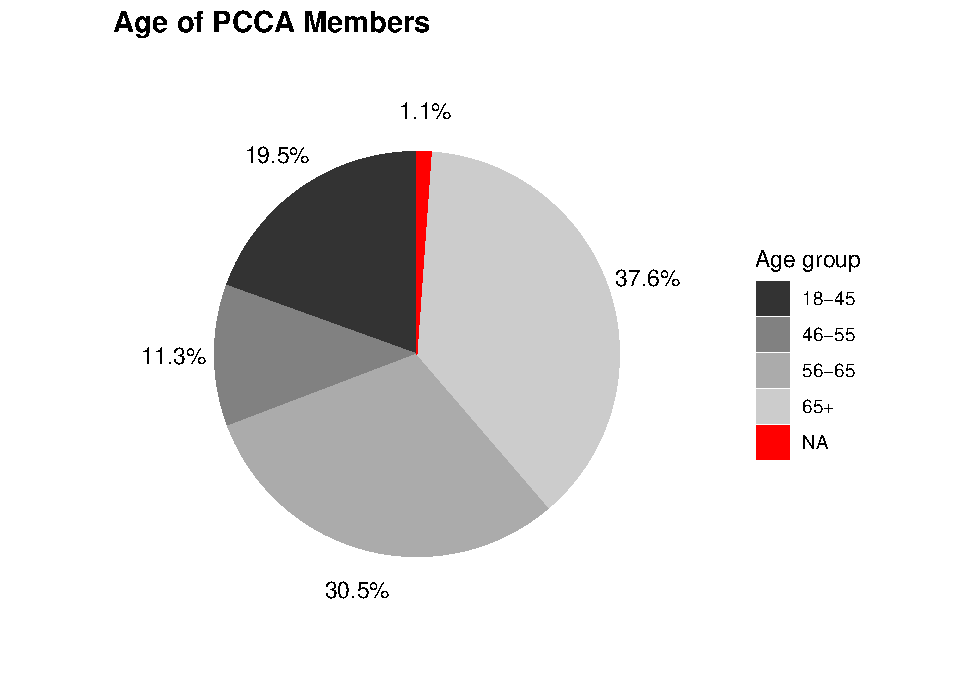
\includegraphics{pcca_survey_files/figure-latex/age-all-1.pdf}

\hypertarget{area-that-members-believe-pcca-performs-best-at}{%
\subsection{Area that members believe PCCA performs best
at}\label{area-that-members-believe-pcca-performs-best-at}}

\begin{Shaded}
\begin{Highlighting}[]
\NormalTok{my.labels }\OtherTok{\textless{}{-}} \FunctionTok{c}\NormalTok{(}\StringTok{"In{-}Person"}\NormalTok{, }\StringTok{"Mass Comm"}\NormalTok{, }\StringTok{"Software/Apps"}\NormalTok{, }\StringTok{"NA"}\NormalTok{)}
\end{Highlighting}
\end{Shaded}

\begin{Shaded}
\begin{Highlighting}[]
\NormalTok{pcca\_best }\OtherTok{\textless{}{-}}\NormalTok{ survey }\SpecialCharTok{\%\textgreater{}\%}
    \FunctionTok{group\_by}\NormalTok{(}\StringTok{\textasciigrave{}}\AttributeTok{area pcca does best}\StringTok{\textasciigrave{}}\NormalTok{) }\SpecialCharTok{\%\textgreater{}\%}
    \FunctionTok{summarise}\NormalTok{(}\AttributeTok{count =} \FunctionTok{n\_distinct}\NormalTok{(number))}

\NormalTok{best }\OtherTok{\textless{}{-}} \FunctionTok{ggplot}\NormalTok{(pcca\_best, }\FunctionTok{aes}\NormalTok{(}\AttributeTok{x =} \StringTok{\textasciigrave{}}\AttributeTok{area pcca does best}\StringTok{\textasciigrave{}}\NormalTok{, }\AttributeTok{y =}\NormalTok{ count)) }\SpecialCharTok{+}
    \FunctionTok{geom\_bar}\NormalTok{(}\AttributeTok{stat =} \StringTok{"identity"}\NormalTok{) }\SpecialCharTok{+} \FunctionTok{coord\_flip}\NormalTok{() }\SpecialCharTok{+} \FunctionTok{ggtitle}\NormalTok{(}\StringTok{"Area That Members Believe PCCA Performs Best"}\NormalTok{)}
\NormalTok{best }\SpecialCharTok{+} \FunctionTok{theme}\NormalTok{(}\AttributeTok{axis.title.y =} \FunctionTok{element\_blank}\NormalTok{(), }\AttributeTok{axis.title.x =} \FunctionTok{element\_blank}\NormalTok{()) }\SpecialCharTok{+}
    \FunctionTok{scale\_x\_discrete}\NormalTok{(}\AttributeTok{labels =}\NormalTok{ my.labels)}
\end{Highlighting}
\end{Shaded}

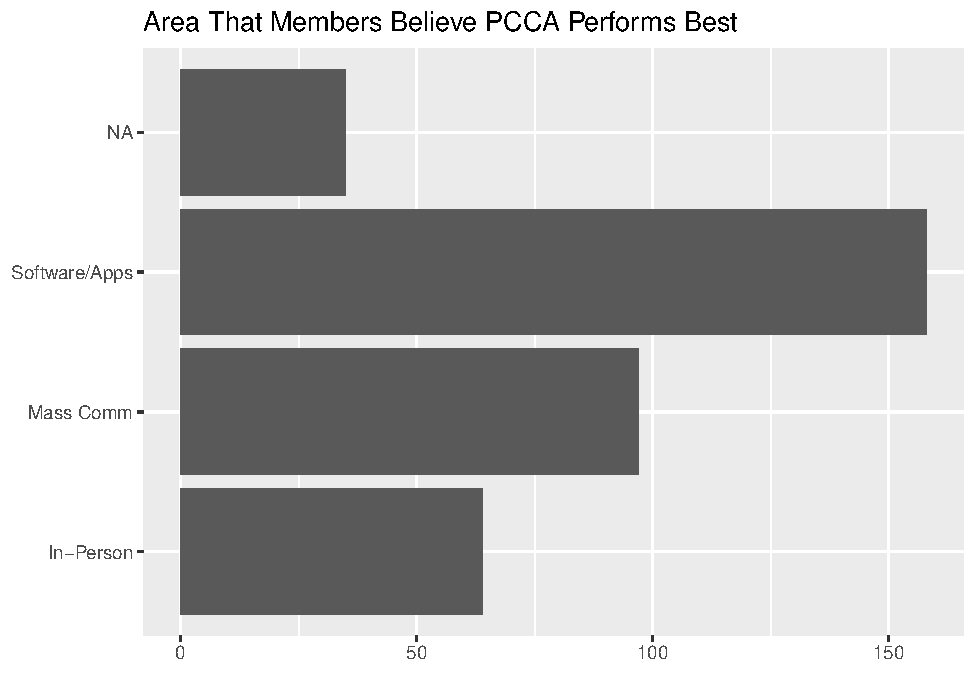
\includegraphics{pcca_survey_files/figure-latex/best-all-1.pdf}

\hypertarget{education}{%
\subsection{Education}\label{education}}

\begin{Shaded}
\begin{Highlighting}[]
\NormalTok{survey }\SpecialCharTok{\%\textgreater{}\%}
    \FunctionTok{group\_by}\NormalTok{(}\StringTok{\textasciigrave{}}\AttributeTok{education level}\StringTok{\textasciigrave{}}\NormalTok{) }\SpecialCharTok{\%\textgreater{}\%}
    \FunctionTok{summarise}\NormalTok{(}\AttributeTok{count =} \FunctionTok{n\_distinct}\NormalTok{(number))}
\end{Highlighting}
\end{Shaded}

\begin{verbatim}
## # A tibble: 20 x 2
##    `education level`                                                  count
##    <chr>                                                              <int>
##  1 College                                                              222
##  2 High School                                                           27
##  3 Other (Please specify):                                                2
##  4 Other (Please specify):6 grade                                         1
##  5 Other (Please specify):BBA & MBA                                       1
##  6 Other (Please specify):does my degree or lack of define my success     1
##  7 Other (Please specify):GED                                             1
##  8 Other (Please specify):graduate degree                                 2
##  9 Other (Please specify):Graduate masters                                1
## 10 Other (Please specify):Graduate school                                 2
## 11 Other (Please specify):Law school                                      1
## 12 Other (Please specify):Master's degree                                 1
## 13 Other (Please specify):Master’s level in Agri                          1
## 14 Other (Please specify):Masters Degree                                  1
## 15 Other (Please specify):MS                                              1
## 16 Other (Please specify):pharmacist                                      1
## 17 Other (Please specify):post graduate degree                            1
## 18 Some College                                                          71
## 19 Trade School                                                          12
## 20 <NA>                                                                   4
\end{verbatim}

\hypertarget{region}{%
\subsection{Region}\label{region}}

\begin{Shaded}
\begin{Highlighting}[]
\NormalTok{region }\OtherTok{\textless{}{-}}\NormalTok{ survey }\SpecialCharTok{\%\textgreater{}\%}
    \FunctionTok{group\_by}\NormalTok{(region) }\SpecialCharTok{\%\textgreater{}\%}
    \FunctionTok{summarise}\NormalTok{(}\AttributeTok{count =} \FunctionTok{n\_distinct}\NormalTok{(number))}

\NormalTok{bp }\OtherTok{\textless{}{-}} \FunctionTok{ggplot}\NormalTok{(region, }\FunctionTok{aes}\NormalTok{(}\AttributeTok{x =} \StringTok{""}\NormalTok{, }\AttributeTok{y =}\NormalTok{ count, }\AttributeTok{fill =}\NormalTok{ region)) }\SpecialCharTok{+}
    \FunctionTok{geom\_bar}\NormalTok{(}\AttributeTok{width =} \DecValTok{1}\NormalTok{, }\AttributeTok{stat =} \StringTok{"identity"}\NormalTok{)}
\NormalTok{pie }\OtherTok{\textless{}{-}}\NormalTok{ bp }\SpecialCharTok{+} \FunctionTok{coord\_polar}\NormalTok{(}\StringTok{"y"}\NormalTok{, }\AttributeTok{start =} \DecValTok{0}\NormalTok{)}

\NormalTok{pie }\SpecialCharTok{+} \FunctionTok{scale\_fill\_grey}\NormalTok{() }\SpecialCharTok{+} \FunctionTok{ggtitle}\NormalTok{(}\StringTok{"PCCA Members Region Location"}\NormalTok{) }\SpecialCharTok{+}
\NormalTok{    blank\_theme }\SpecialCharTok{+} \FunctionTok{theme}\NormalTok{(}\AttributeTok{axis.text.x =} \FunctionTok{element\_blank}\NormalTok{()) }\SpecialCharTok{+} \FunctionTok{geom\_text}\NormalTok{(}\FunctionTok{aes}\NormalTok{(}\AttributeTok{x =} \FloatTok{1.7}\NormalTok{,}
    \AttributeTok{label =} \FunctionTok{percent}\NormalTok{(count}\SpecialCharTok{/}\DecValTok{354}\NormalTok{, }\AttributeTok{accuracy =} \FloatTok{0.1}\NormalTok{)), }\AttributeTok{position =} \FunctionTok{position\_stack}\NormalTok{(}\AttributeTok{vjust =} \FloatTok{0.5}\NormalTok{)) }\SpecialCharTok{+}
    \FunctionTok{guides}\NormalTok{(}\AttributeTok{fill =} \FunctionTok{guide\_legend}\NormalTok{(}\AttributeTok{title =} \StringTok{"Region"}\NormalTok{))}
\end{Highlighting}
\end{Shaded}

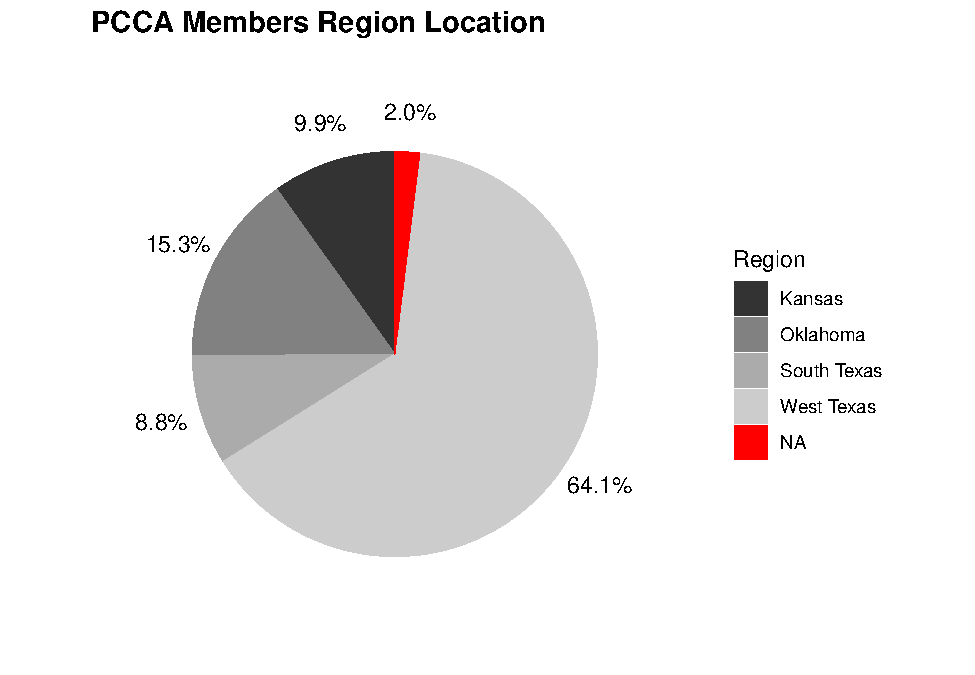
\includegraphics{pcca_survey_files/figure-latex/region-all-1.pdf}

\hypertarget{preferred-information}{%
\subsection{Preferred Information}\label{preferred-information}}

\begin{Shaded}
\begin{Highlighting}[]
\NormalTok{information }\OtherTok{\textless{}{-}}\NormalTok{ survey }\SpecialCharTok{\%\textgreater{}\%}
    \FunctionTok{group\_by}\NormalTok{(}\StringTok{\textasciigrave{}}\AttributeTok{gathering information}\StringTok{\textasciigrave{}}\NormalTok{) }\SpecialCharTok{\%\textgreater{}\%}
    \FunctionTok{summarise}\NormalTok{(}\AttributeTok{count =} \FunctionTok{n\_distinct}\NormalTok{(number))}

\NormalTok{information }\OtherTok{\textless{}{-}}\NormalTok{ information }\SpecialCharTok{\%\textgreater{}\%}
    \FunctionTok{filter}\NormalTok{(information}\SpecialCharTok{$}\NormalTok{count }\SpecialCharTok{\textgreater{}} \DecValTok{4}\NormalTok{)}

\NormalTok{total }\OtherTok{\textless{}{-}} \FunctionTok{as.numeric}\NormalTok{(}\FunctionTok{nrow}\NormalTok{(survey))}

\NormalTok{bp }\OtherTok{\textless{}{-}} \FunctionTok{ggplot}\NormalTok{(information, }\FunctionTok{aes}\NormalTok{(}\AttributeTok{x =} \StringTok{""}\NormalTok{, }\AttributeTok{y =}\NormalTok{ count, }\AttributeTok{fill =} \StringTok{\textasciigrave{}}\AttributeTok{gathering information}\StringTok{\textasciigrave{}}\NormalTok{)) }\SpecialCharTok{+}
    \FunctionTok{geom\_bar}\NormalTok{(}\AttributeTok{width =} \DecValTok{1}\NormalTok{, }\AttributeTok{stat =} \StringTok{"identity"}\NormalTok{)}
\NormalTok{pie }\OtherTok{\textless{}{-}}\NormalTok{ bp }\SpecialCharTok{+} \FunctionTok{coord\_polar}\NormalTok{(}\StringTok{"y"}\NormalTok{, }\AttributeTok{start =} \DecValTok{0}\NormalTok{)}

\NormalTok{pie }\SpecialCharTok{+} \FunctionTok{scale\_fill\_grey}\NormalTok{() }\SpecialCharTok{+} \FunctionTok{ggtitle}\NormalTok{(}\StringTok{"PCCA Members Preferred Information Sources"}\NormalTok{) }\SpecialCharTok{+}
\NormalTok{    blank\_theme }\SpecialCharTok{+} \FunctionTok{theme}\NormalTok{(}\AttributeTok{axis.text.x =} \FunctionTok{element\_blank}\NormalTok{()) }\SpecialCharTok{+} \FunctionTok{geom\_text}\NormalTok{(}\FunctionTok{aes}\NormalTok{(}\AttributeTok{x =} \FloatTok{1.7}\NormalTok{,}
    \AttributeTok{label =} \FunctionTok{percent}\NormalTok{(count}\SpecialCharTok{/}\NormalTok{total, }\AttributeTok{accuracy =} \FloatTok{0.1}\NormalTok{)), }\AttributeTok{position =} \FunctionTok{position\_stack}\NormalTok{(}\AttributeTok{vjust =} \FloatTok{0.5}\NormalTok{)) }\SpecialCharTok{+}
    \FunctionTok{guides}\NormalTok{(}\AttributeTok{fill =} \FunctionTok{guide\_legend}\NormalTok{(}\AttributeTok{title =} \StringTok{"Types of sources"}\NormalTok{))}
\end{Highlighting}
\end{Shaded}

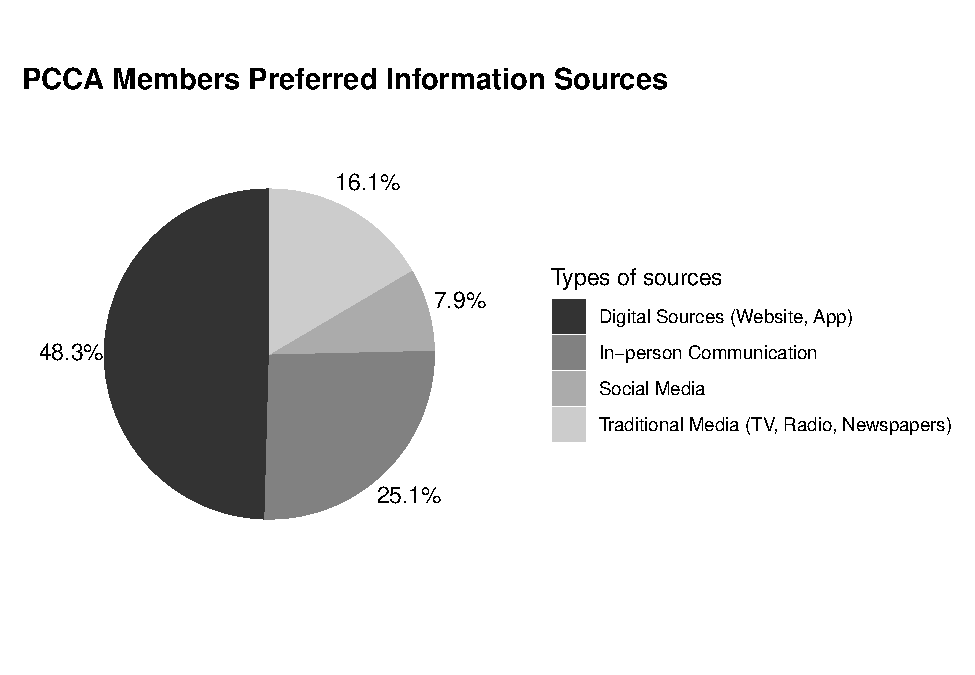
\includegraphics{pcca_survey_files/figure-latex/preferred-all-1.pdf}

\hypertarget{dry-or-irrigated-operation}{%
\subsection{Dry or Irrigated
Operation}\label{dry-or-irrigated-operation}}

\begin{Shaded}
\begin{Highlighting}[]
\NormalTok{operation }\OtherTok{\textless{}{-}}\NormalTok{ survey }\SpecialCharTok{\%\textgreater{}\%}
    \FunctionTok{group\_by}\NormalTok{(operation) }\SpecialCharTok{\%\textgreater{}\%}
    \FunctionTok{summarise}\NormalTok{(}\AttributeTok{count =} \FunctionTok{n\_distinct}\NormalTok{(number))}


\NormalTok{bp }\OtherTok{\textless{}{-}} \FunctionTok{ggplot}\NormalTok{(operation, }\FunctionTok{aes}\NormalTok{(}\AttributeTok{x =} \StringTok{""}\NormalTok{, }\AttributeTok{y =}\NormalTok{ count, }\AttributeTok{fill =}\NormalTok{ operation)) }\SpecialCharTok{+}
    \FunctionTok{geom\_bar}\NormalTok{(}\AttributeTok{width =} \DecValTok{1}\NormalTok{, }\AttributeTok{stat =} \StringTok{"identity"}\NormalTok{)}
\NormalTok{pie }\OtherTok{\textless{}{-}}\NormalTok{ bp }\SpecialCharTok{+} \FunctionTok{coord\_polar}\NormalTok{(}\StringTok{"y"}\NormalTok{, }\AttributeTok{start =} \DecValTok{0}\NormalTok{)}

\NormalTok{pie }\SpecialCharTok{+} \FunctionTok{scale\_fill\_grey}\NormalTok{() }\SpecialCharTok{+} \FunctionTok{ggtitle}\NormalTok{(}\StringTok{"Dry or Irrigated Operation"}\NormalTok{) }\SpecialCharTok{+}
\NormalTok{    blank\_theme }\SpecialCharTok{+} \FunctionTok{theme}\NormalTok{(}\AttributeTok{axis.text.x =} \FunctionTok{element\_blank}\NormalTok{()) }\SpecialCharTok{+} \FunctionTok{geom\_text}\NormalTok{(}\FunctionTok{aes}\NormalTok{(}\AttributeTok{x =} \FloatTok{1.7}\NormalTok{,}
    \AttributeTok{label =} \FunctionTok{percent}\NormalTok{(count}\SpecialCharTok{/}\DecValTok{354}\NormalTok{, }\AttributeTok{accuracy =} \FloatTok{0.1}\NormalTok{)), }\AttributeTok{position =} \FunctionTok{position\_stack}\NormalTok{(}\AttributeTok{vjust =} \FloatTok{0.5}\NormalTok{)) }\SpecialCharTok{+}
    \FunctionTok{guides}\NormalTok{(}\AttributeTok{fill =} \FunctionTok{guide\_legend}\NormalTok{(}\AttributeTok{title =} \StringTok{"Types of operation"}\NormalTok{))}
\end{Highlighting}
\end{Shaded}

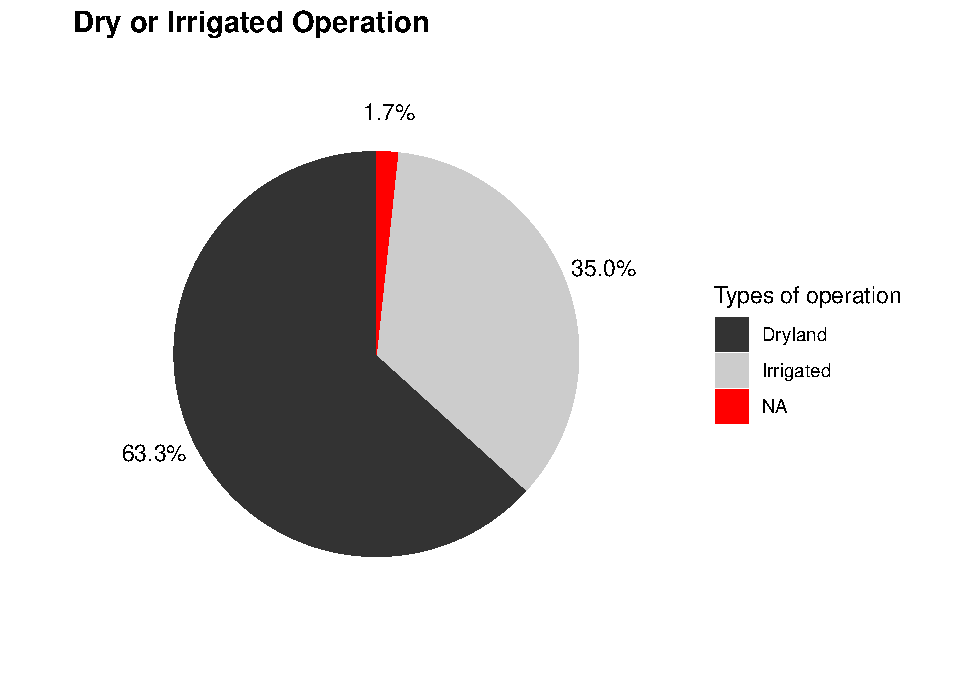
\includegraphics{pcca_survey_files/figure-latex/operation-all-1.pdf}

\begin{Shaded}
\begin{Highlighting}[]
\NormalTok{meetings }\OtherTok{\textless{}{-}}\NormalTok{ survey }\SpecialCharTok{\%\textgreater{}\%}
    \FunctionTok{group\_by}\NormalTok{(}\StringTok{\textasciigrave{}}\AttributeTok{coop meetings}\StringTok{\textasciigrave{}}\NormalTok{) }\SpecialCharTok{\%\textgreater{}\%}
    \FunctionTok{summarise}\NormalTok{(}\AttributeTok{count =} \FunctionTok{n\_distinct}\NormalTok{(number))}

\NormalTok{meetings\_chart }\OtherTok{\textless{}{-}} \FunctionTok{ggplot}\NormalTok{(meetings, }\FunctionTok{aes}\NormalTok{(}\AttributeTok{x =} \StringTok{\textasciigrave{}}\AttributeTok{coop meetings}\StringTok{\textasciigrave{}}\NormalTok{, }\AttributeTok{y =}\NormalTok{ count)) }\SpecialCharTok{+}
    \FunctionTok{geom\_bar}\NormalTok{(}\AttributeTok{stat =} \StringTok{"identity"}\NormalTok{) }\SpecialCharTok{+} \FunctionTok{coord\_flip}\NormalTok{() }\SpecialCharTok{+} \FunctionTok{ggtitle}\NormalTok{(}\StringTok{"Frequency of Attendance at PCCA Meetings"}\NormalTok{)}
\NormalTok{meetings\_chart }\SpecialCharTok{+} \FunctionTok{theme}\NormalTok{(}\AttributeTok{axis.title.y =} \FunctionTok{element\_blank}\NormalTok{(), }\AttributeTok{axis.title.x =} \FunctionTok{element\_blank}\NormalTok{())}
\end{Highlighting}
\end{Shaded}

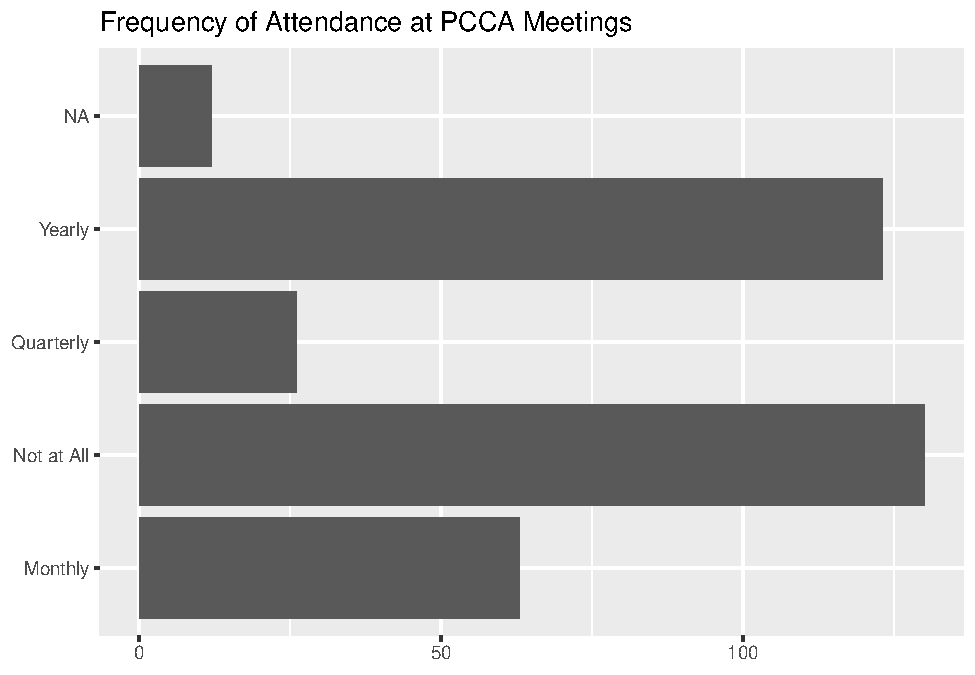
\includegraphics{pcca_survey_files/figure-latex/meetings-all-1.pdf}

\hypertarget{most-used-marketing-method}{%
\subsection{Most used marketing
method}\label{most-used-marketing-method}}

\begin{Shaded}
\begin{Highlighting}[]
\NormalTok{marketing }\OtherTok{\textless{}{-}}\NormalTok{ survey }\SpecialCharTok{\%\textgreater{}\%}
    \FunctionTok{group\_by}\NormalTok{(}\StringTok{\textasciigrave{}}\AttributeTok{most used marketing method}\StringTok{\textasciigrave{}}\NormalTok{) }\SpecialCharTok{\%\textgreater{}\%}
    \FunctionTok{summarise}\NormalTok{(}\AttributeTok{count =} \FunctionTok{n\_distinct}\NormalTok{(number))}

\NormalTok{lbls }\OtherTok{\textless{}{-}} \FunctionTok{paste}\NormalTok{(}\FunctionTok{names}\NormalTok{(marketing), }\StringTok{"}\SpecialCharTok{\textbackslash{}n}\StringTok{"}\NormalTok{, marketing, }\AttributeTok{sep =} \StringTok{""}\NormalTok{)}

\NormalTok{total }\OtherTok{\textless{}{-}} \FunctionTok{as.numeric}\NormalTok{(}\FunctionTok{nrow}\NormalTok{(survey))}

\NormalTok{bp }\OtherTok{\textless{}{-}} \FunctionTok{ggplot}\NormalTok{(marketing, }\FunctionTok{aes}\NormalTok{(}\AttributeTok{x =} \StringTok{""}\NormalTok{, }\AttributeTok{y =}\NormalTok{ count, }\AttributeTok{fill =} \StringTok{\textasciigrave{}}\AttributeTok{most used marketing method}\StringTok{\textasciigrave{}}\NormalTok{)) }\SpecialCharTok{+}
    \FunctionTok{geom\_bar}\NormalTok{(}\AttributeTok{width =} \DecValTok{1}\NormalTok{, }\AttributeTok{stat =} \StringTok{"identity"}\NormalTok{)}
\NormalTok{pie }\OtherTok{\textless{}{-}}\NormalTok{ bp }\SpecialCharTok{+} \FunctionTok{coord\_polar}\NormalTok{(}\StringTok{"y"}\NormalTok{, }\AttributeTok{start =} \DecValTok{0}\NormalTok{)}

\NormalTok{pie }\SpecialCharTok{+} \FunctionTok{ggtitle}\NormalTok{(}\StringTok{"Most Used Marketing Method"}\NormalTok{) }\SpecialCharTok{+}\NormalTok{ blank\_theme }\SpecialCharTok{+} \FunctionTok{theme}\NormalTok{(}\AttributeTok{axis.text.x =} \FunctionTok{element\_blank}\NormalTok{()) }\SpecialCharTok{+}
    \FunctionTok{geom\_text}\NormalTok{(}\FunctionTok{aes}\NormalTok{(}\AttributeTok{x =} \FloatTok{1.7}\NormalTok{, }\AttributeTok{label =} \FunctionTok{percent}\NormalTok{(count}\SpecialCharTok{/}\NormalTok{total, }\AttributeTok{accuracy =} \FloatTok{0.1}\NormalTok{)),}
        \AttributeTok{position =} \FunctionTok{position\_stack}\NormalTok{(}\AttributeTok{vjust =} \FloatTok{0.5}\NormalTok{)) }\SpecialCharTok{+} \FunctionTok{guides}\NormalTok{(}\AttributeTok{fill =} \FunctionTok{guide\_legend}\NormalTok{(}\AttributeTok{title =} \StringTok{"Marketing methods"}\NormalTok{))}
\end{Highlighting}
\end{Shaded}

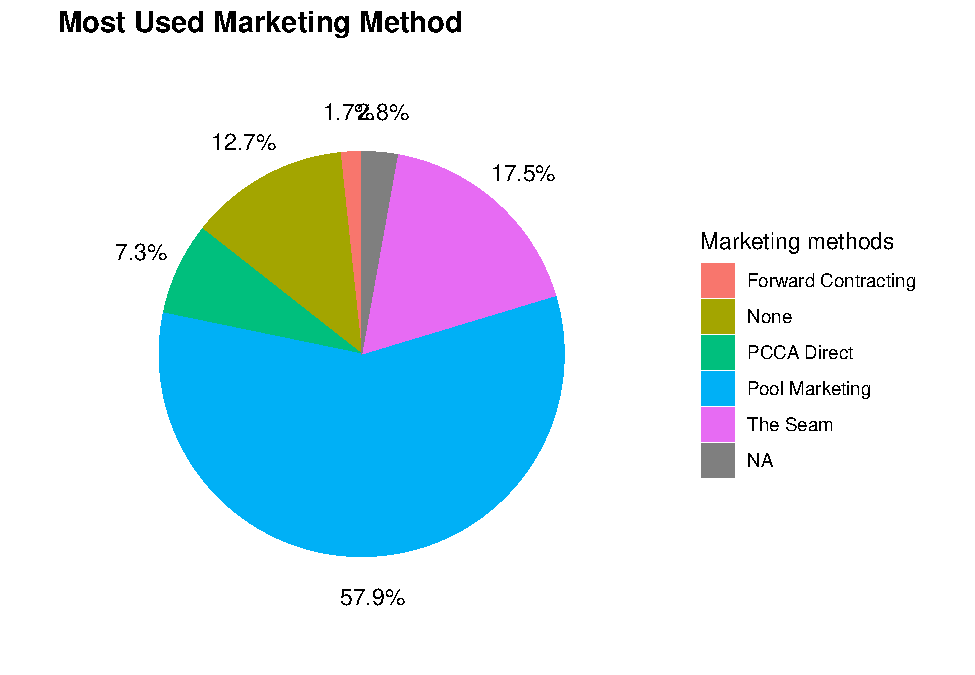
\includegraphics{pcca_survey_files/figure-latex/most-used-all-1.pdf}

\begin{Shaded}
\begin{Highlighting}[]
\NormalTok{tenant }\OtherTok{\textless{}{-}}\NormalTok{ survey }\SpecialCharTok{\%\textgreater{}\%}
    \FunctionTok{group\_by}\NormalTok{(description) }\SpecialCharTok{\%\textgreater{}\%}
    \FunctionTok{summarise}\NormalTok{(}\AttributeTok{count =} \FunctionTok{n\_distinct}\NormalTok{(number))}

\NormalTok{total }\OtherTok{\textless{}{-}} \FunctionTok{as.numeric}\NormalTok{(}\FunctionTok{nrow}\NormalTok{(survey))}

\NormalTok{bp }\OtherTok{\textless{}{-}} \FunctionTok{ggplot}\NormalTok{(tenant, }\FunctionTok{aes}\NormalTok{(}\AttributeTok{x =} \StringTok{""}\NormalTok{, }\AttributeTok{y =}\NormalTok{ count, }\AttributeTok{fill =}\NormalTok{ description)) }\SpecialCharTok{+}
    \FunctionTok{geom\_bar}\NormalTok{(}\AttributeTok{width =} \DecValTok{1}\NormalTok{, }\AttributeTok{stat =} \StringTok{"identity"}\NormalTok{)}
\NormalTok{pie }\OtherTok{\textless{}{-}}\NormalTok{ bp }\SpecialCharTok{+} \FunctionTok{coord\_polar}\NormalTok{(}\StringTok{"y"}\NormalTok{, }\AttributeTok{start =} \DecValTok{0}\NormalTok{)}

\NormalTok{pie }\SpecialCharTok{+} \FunctionTok{scale\_fill\_grey}\NormalTok{() }\SpecialCharTok{+} \FunctionTok{ggtitle}\NormalTok{(}\StringTok{"Tenant or Landlord"}\NormalTok{) }\SpecialCharTok{+}\NormalTok{ blank\_theme }\SpecialCharTok{+}
    \FunctionTok{theme}\NormalTok{(}\AttributeTok{axis.text.x =} \FunctionTok{element\_blank}\NormalTok{()) }\SpecialCharTok{+} \FunctionTok{geom\_text}\NormalTok{(}\FunctionTok{aes}\NormalTok{(}\AttributeTok{x =} \FloatTok{1.7}\NormalTok{,}
    \AttributeTok{label =} \FunctionTok{percent}\NormalTok{(count}\SpecialCharTok{/}\NormalTok{total, }\AttributeTok{accuracy =} \FloatTok{0.1}\NormalTok{)), }\AttributeTok{position =} \FunctionTok{position\_stack}\NormalTok{(}\AttributeTok{vjust =} \FloatTok{0.5}\NormalTok{)) }\SpecialCharTok{+}
    \FunctionTok{guides}\NormalTok{(}\AttributeTok{fill =} \FunctionTok{guide\_legend}\NormalTok{(}\AttributeTok{title =} \StringTok{"Management"}\NormalTok{))}
\end{Highlighting}
\end{Shaded}

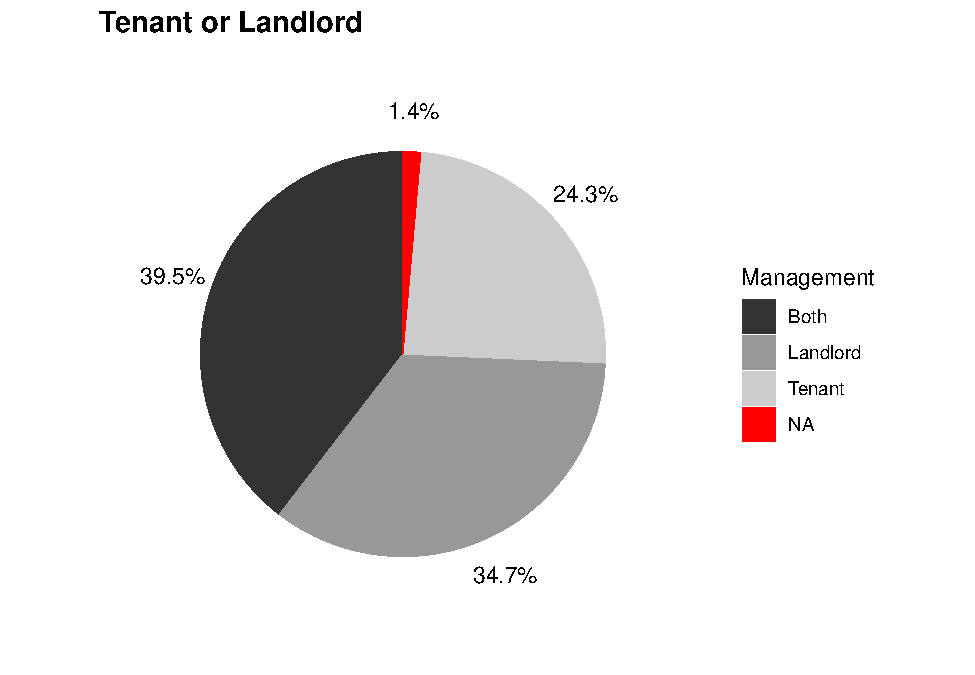
\includegraphics{pcca_survey_files/figure-latex/tenant-all-1.pdf}

\hypertarget{data-analysis}{%
\section{Data analysis}\label{data-analysis}}

Prediction of membership satisfaction

\begin{Shaded}
\begin{Highlighting}[]
\NormalTok{satisfaction }\OtherTok{=} \FunctionTok{lm}\NormalTok{(satisfaction }\SpecialCharTok{\textasciitilde{}}\NormalTok{ accessible }\SpecialCharTok{+}\NormalTok{ responsive }\SpecialCharTok{+}\NormalTok{ courteous,}
    \AttributeTok{data =}\NormalTok{ survey)}
\FunctionTok{stargazer}\NormalTok{(satisfaction)}
\end{Highlighting}
\end{Shaded}

\begin{verbatim}
## 
## % Table created by stargazer v.5.2.3 by Marek Hlavac, Social Policy Institute. E-mail: marek.hlavac at gmail.com
## % Date and time: Wed, Apr 20, 2022 - 8:02:46 AM
## \begin{table}[!htbp] \centering 
##   \caption{} 
##   \label{} 
## \begin{tabular}{@{\extracolsep{5pt}}lc} 
## \\[-1.8ex]\hline 
## \hline \\[-1.8ex] 
##  & \multicolumn{1}{c}{\textit{Dependent variable:}} \\ 
## \cline{2-2} 
## \\[-1.8ex] & satisfaction \\ 
## \hline \\[-1.8ex] 
##  accessible & 0.266$^{**}$ \\ 
##   & (0.107) \\ 
##   & \\ 
##  responsive & 0.452$^{***}$ \\ 
##   & (0.128) \\ 
##   & \\ 
##  courteous & 0.107 \\ 
##   & (0.107) \\ 
##   & \\ 
##  Constant & 0.369 \\ 
##   & (0.357) \\ 
##   & \\ 
## \hline \\[-1.8ex] 
## Observations & 329 \\ 
## R$^{2}$ & 0.317 \\ 
## Adjusted R$^{2}$ & 0.310 \\ 
## Residual Std. Error & 1.059 (df = 325) \\ 
## F Statistic & 50.194$^{***}$ (df = 3; 325) \\ 
## \hline 
## \hline \\[-1.8ex] 
## \textit{Note:}  & \multicolumn{1}{r}{$^{*}$p$<$0.1; $^{**}$p$<$0.05; $^{***}$p$<$0.01} \\ 
## \end{tabular} 
## \end{table}
\end{verbatim}

\begin{Shaded}
\begin{Highlighting}[]
\NormalTok{satisfaction2 }\OtherTok{=} \FunctionTok{lm}\NormalTok{(satisfaction }\SpecialCharTok{\textasciitilde{}}\NormalTok{ accessible }\SpecialCharTok{+}\NormalTok{ responsive }\SpecialCharTok{+}\NormalTok{ courteous }\SpecialCharTok{+}
    \StringTok{\textasciigrave{}}\AttributeTok{marketing pool}\StringTok{\textasciigrave{}} \SpecialCharTok{+} \StringTok{\textasciigrave{}}\AttributeTok{the seam}\StringTok{\textasciigrave{}} \SpecialCharTok{+} \StringTok{\textasciigrave{}}\AttributeTok{pcca direct}\StringTok{\textasciigrave{}} \SpecialCharTok{+} \StringTok{\textasciigrave{}}\AttributeTok{forward contracting}\StringTok{\textasciigrave{}}\NormalTok{,}
    \AttributeTok{data =}\NormalTok{ survey)}
\FunctionTok{stargazer}\NormalTok{(satisfaction2)}
\end{Highlighting}
\end{Shaded}

\begin{verbatim}
## 
## % Table created by stargazer v.5.2.3 by Marek Hlavac, Social Policy Institute. E-mail: marek.hlavac at gmail.com
## % Date and time: Wed, Apr 20, 2022 - 8:02:46 AM
## \begin{table}[!htbp] \centering 
##   \caption{} 
##   \label{} 
## \begin{tabular}{@{\extracolsep{5pt}}lc} 
## \\[-1.8ex]\hline 
## \hline \\[-1.8ex] 
##  & \multicolumn{1}{c}{\textit{Dependent variable:}} \\ 
## \cline{2-2} 
## \\[-1.8ex] & satisfaction \\ 
## \hline \\[-1.8ex] 
##  accessible & 0.293$^{***}$ \\ 
##   & (0.106) \\ 
##   & \\ 
##  responsive & 0.378$^{***}$ \\ 
##   & (0.129) \\ 
##   & \\ 
##  courteous & 0.168 \\ 
##   & (0.107) \\ 
##   & \\ 
##  `marketing pool` & 0.005 \\ 
##   & (0.119) \\ 
##   & \\ 
##  `the seam` & $-$0.242$^{**}$ \\ 
##   & (0.117) \\ 
##   & \\ 
##  `pcca direct` & 0.281$^{**}$ \\ 
##   & (0.115) \\ 
##   & \\ 
##  `forward contracting` & $-$0.110 \\ 
##   & (0.126) \\ 
##   & \\ 
##  Constant & 0.452 \\ 
##   & (0.415) \\ 
##   & \\ 
## \hline \\[-1.8ex] 
## Observations & 311 \\ 
## R$^{2}$ & 0.369 \\ 
## Adjusted R$^{2}$ & 0.354 \\ 
## Residual Std. Error & 1.024 (df = 303) \\ 
## F Statistic & 25.267$^{***}$ (df = 7; 303) \\ 
## \hline 
## \hline \\[-1.8ex] 
## \textit{Note:}  & \multicolumn{1}{r}{$^{*}$p$<$0.1; $^{**}$p$<$0.05; $^{***}$p$<$0.01} \\ 
## \end{tabular} 
## \end{table}
\end{verbatim}

\hypertarget{separating-younger-and-older-generation}{%
\section{Separating younger and older
generation}\label{separating-younger-and-older-generation}}

In this section, I will categorize the younger generation as the age
bracket 18-45 and the older generation as the age brackets for 56-65 and
65+

\begin{Shaded}
\begin{Highlighting}[]
\NormalTok{younger }\OtherTok{\textless{}{-}}\NormalTok{ survey }\SpecialCharTok{\%\textgreater{}\%}
    \FunctionTok{filter}\NormalTok{(survey}\SpecialCharTok{$}\NormalTok{age }\SpecialCharTok{==} \StringTok{"18{-}45"}\NormalTok{)}

\NormalTok{older }\OtherTok{\textless{}{-}}\NormalTok{ survey }\SpecialCharTok{\%\textgreater{}\%}
    \FunctionTok{filter}\NormalTok{(survey}\SpecialCharTok{$}\NormalTok{age }\SpecialCharTok{==} \StringTok{"56{-}65"} \SpecialCharTok{|}\NormalTok{ survey}\SpecialCharTok{$}\NormalTok{age }\SpecialCharTok{==} \StringTok{"65+"}\NormalTok{)}

\NormalTok{younger}\SpecialCharTok{$}\NormalTok{gen }\OtherTok{\textless{}{-}} \StringTok{"younger"}
\NormalTok{older}\SpecialCharTok{$}\NormalTok{gen }\OtherTok{\textless{}{-}} \StringTok{"older"}
\end{Highlighting}
\end{Shaded}

\begin{Shaded}
\begin{Highlighting}[]
\NormalTok{satisfaction.y }\OtherTok{=} \FunctionTok{lm}\NormalTok{(satisfaction }\SpecialCharTok{\textasciitilde{}}\NormalTok{ accessible }\SpecialCharTok{+}\NormalTok{ responsive }\SpecialCharTok{+}
\NormalTok{    courteous, }\AttributeTok{data =}\NormalTok{ older)}
\FunctionTok{stargazer}\NormalTok{(satisfaction.y)}
\end{Highlighting}
\end{Shaded}

\begin{verbatim}
## 
## % Table created by stargazer v.5.2.3 by Marek Hlavac, Social Policy Institute. E-mail: marek.hlavac at gmail.com
## % Date and time: Wed, Apr 20, 2022 - 8:02:46 AM
## \begin{table}[!htbp] \centering 
##   \caption{} 
##   \label{} 
## \begin{tabular}{@{\extracolsep{5pt}}lc} 
## \\[-1.8ex]\hline 
## \hline \\[-1.8ex] 
##  & \multicolumn{1}{c}{\textit{Dependent variable:}} \\ 
## \cline{2-2} 
## \\[-1.8ex] & satisfaction \\ 
## \hline \\[-1.8ex] 
##  accessible & 0.296$^{**}$ \\ 
##   & (0.120) \\ 
##   & \\ 
##  responsive & 0.378$^{**}$ \\ 
##   & (0.154) \\ 
##   & \\ 
##  courteous & 0.193 \\ 
##   & (0.130) \\ 
##   & \\ 
##  Constant & 0.253 \\ 
##   & (0.417) \\ 
##   & \\ 
## \hline \\[-1.8ex] 
## Observations & 221 \\ 
## R$^{2}$ & 0.362 \\ 
## Adjusted R$^{2}$ & 0.353 \\ 
## Residual Std. Error & 1.030 (df = 217) \\ 
## F Statistic & 41.078$^{***}$ (df = 3; 217) \\ 
## \hline 
## \hline \\[-1.8ex] 
## \textit{Note:}  & \multicolumn{1}{r}{$^{*}$p$<$0.1; $^{**}$p$<$0.05; $^{***}$p$<$0.01} \\ 
## \end{tabular} 
## \end{table}
\end{verbatim}

\begin{Shaded}
\begin{Highlighting}[]
\NormalTok{pcca\_best }\OtherTok{\textless{}{-}}\NormalTok{ younger }\SpecialCharTok{\%\textgreater{}\%}
    \FunctionTok{group\_by}\NormalTok{(}\StringTok{\textasciigrave{}}\AttributeTok{area pcca does best}\StringTok{\textasciigrave{}}\NormalTok{) }\SpecialCharTok{\%\textgreater{}\%}
    \FunctionTok{summarise}\NormalTok{(}\AttributeTok{count =} \FunctionTok{n\_distinct}\NormalTok{(number))}

\NormalTok{best }\OtherTok{\textless{}{-}} \FunctionTok{ggplot}\NormalTok{(pcca\_best, }\FunctionTok{aes}\NormalTok{(}\AttributeTok{x =} \StringTok{\textasciigrave{}}\AttributeTok{area pcca does best}\StringTok{\textasciigrave{}}\NormalTok{, }\AttributeTok{y =}\NormalTok{ count)) }\SpecialCharTok{+}
    \FunctionTok{geom\_bar}\NormalTok{(}\AttributeTok{stat =} \StringTok{"identity"}\NormalTok{) }\SpecialCharTok{+} \FunctionTok{coord\_flip}\NormalTok{() }\SpecialCharTok{+} \FunctionTok{ggtitle}\NormalTok{(}\StringTok{"Area That Younger Members Believe PCCA Performs Best"}\NormalTok{)}
\NormalTok{best }\SpecialCharTok{+} \FunctionTok{theme}\NormalTok{(}\AttributeTok{axis.title.y =} \FunctionTok{element\_blank}\NormalTok{(), }\AttributeTok{axis.title.x =} \FunctionTok{element\_blank}\NormalTok{()) }\SpecialCharTok{+}
    \FunctionTok{scale\_x\_discrete}\NormalTok{(}\AttributeTok{labels =}\NormalTok{ my.labels)}
\end{Highlighting}
\end{Shaded}

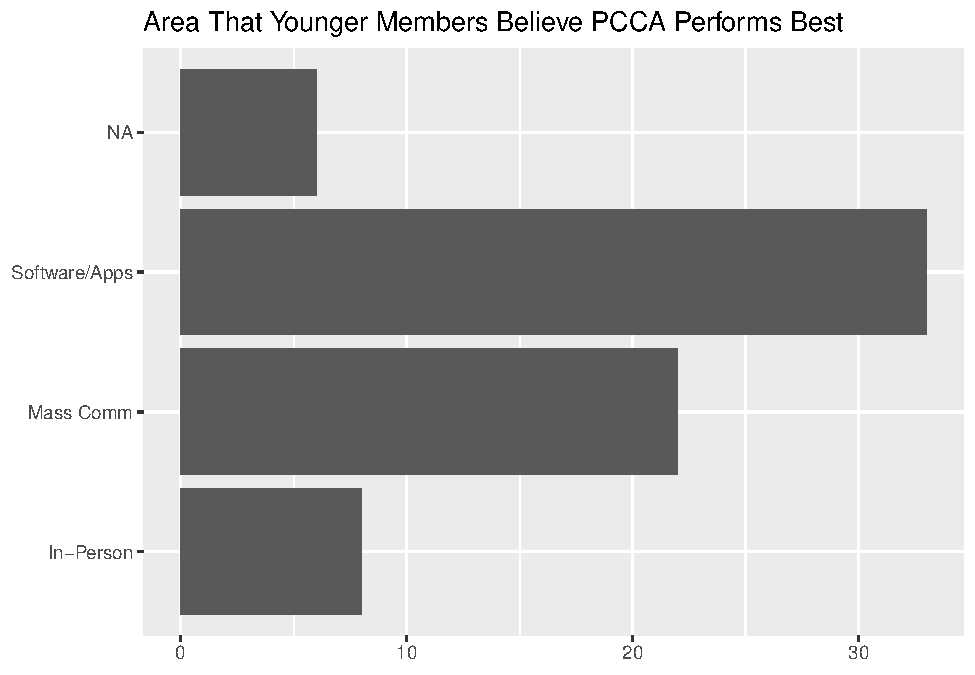
\includegraphics{pcca_survey_files/figure-latex/best-young-1.pdf}

\begin{Shaded}
\begin{Highlighting}[]
\NormalTok{pcca\_best }\OtherTok{\textless{}{-}}\NormalTok{ older }\SpecialCharTok{\%\textgreater{}\%}
    \FunctionTok{group\_by}\NormalTok{(}\StringTok{\textasciigrave{}}\AttributeTok{area pcca does best}\StringTok{\textasciigrave{}}\NormalTok{) }\SpecialCharTok{\%\textgreater{}\%}
    \FunctionTok{summarise}\NormalTok{(}\AttributeTok{count =} \FunctionTok{n\_distinct}\NormalTok{(number))}

\NormalTok{best }\OtherTok{\textless{}{-}} \FunctionTok{ggplot}\NormalTok{(pcca\_best, }\FunctionTok{aes}\NormalTok{(}\AttributeTok{x =} \StringTok{\textasciigrave{}}\AttributeTok{area pcca does best}\StringTok{\textasciigrave{}}\NormalTok{, }\AttributeTok{y =}\NormalTok{ count)) }\SpecialCharTok{+}
    \FunctionTok{geom\_bar}\NormalTok{(}\AttributeTok{stat =} \StringTok{"identity"}\NormalTok{) }\SpecialCharTok{+} \FunctionTok{coord\_flip}\NormalTok{() }\SpecialCharTok{+} \FunctionTok{ggtitle}\NormalTok{(}\StringTok{"Area That Older Members Believe PCCA Performs Best"}\NormalTok{)}
\NormalTok{best }\SpecialCharTok{+} \FunctionTok{theme}\NormalTok{(}\AttributeTok{axis.title.y =} \FunctionTok{element\_blank}\NormalTok{(), }\AttributeTok{axis.title.x =} \FunctionTok{element\_blank}\NormalTok{()) }\SpecialCharTok{+}
    \FunctionTok{scale\_x\_discrete}\NormalTok{(}\AttributeTok{labels =}\NormalTok{ my.labels)}
\end{Highlighting}
\end{Shaded}

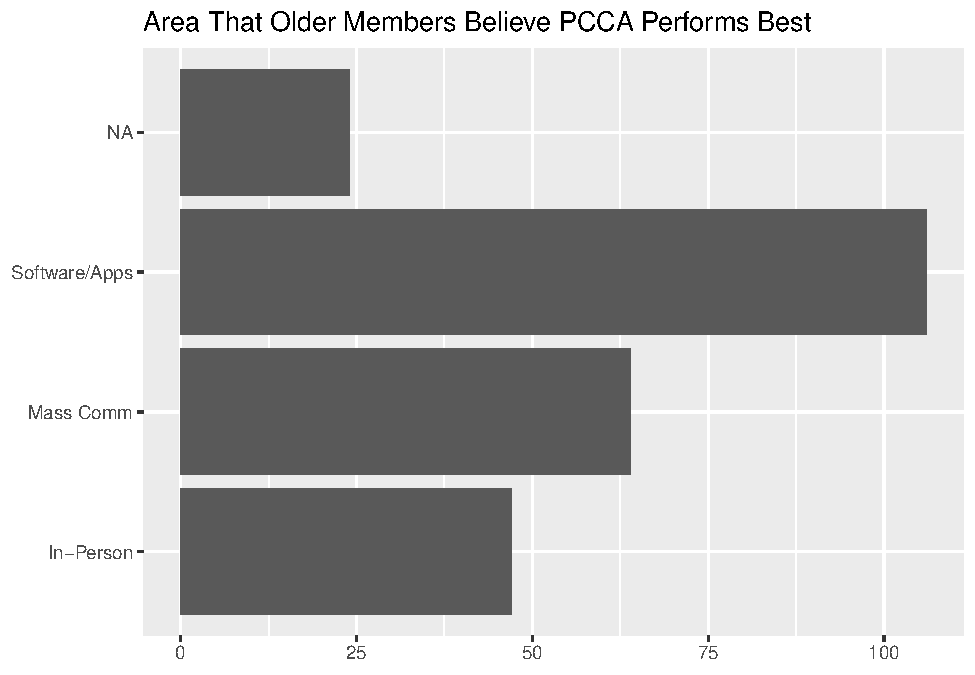
\includegraphics{pcca_survey_files/figure-latex/best-old-1.pdf}

\begin{Shaded}
\begin{Highlighting}[]
\NormalTok{region }\OtherTok{\textless{}{-}}\NormalTok{ younger }\SpecialCharTok{\%\textgreater{}\%}
    \FunctionTok{group\_by}\NormalTok{(region) }\SpecialCharTok{\%\textgreater{}\%}
    \FunctionTok{summarise}\NormalTok{(}\AttributeTok{count =} \FunctionTok{n\_distinct}\NormalTok{(number))}

\NormalTok{bp }\OtherTok{\textless{}{-}} \FunctionTok{ggplot}\NormalTok{(region, }\FunctionTok{aes}\NormalTok{(}\AttributeTok{x =} \StringTok{""}\NormalTok{, }\AttributeTok{y =}\NormalTok{ count, }\AttributeTok{fill =}\NormalTok{ region)) }\SpecialCharTok{+}
    \FunctionTok{geom\_bar}\NormalTok{(}\AttributeTok{width =} \DecValTok{1}\NormalTok{, }\AttributeTok{stat =} \StringTok{"identity"}\NormalTok{)}
\NormalTok{pie }\OtherTok{\textless{}{-}}\NormalTok{ bp }\SpecialCharTok{+} \FunctionTok{coord\_polar}\NormalTok{(}\StringTok{"y"}\NormalTok{, }\AttributeTok{start =} \DecValTok{0}\NormalTok{)}

\NormalTok{total }\OtherTok{\textless{}{-}} \FunctionTok{as.numeric}\NormalTok{(}\FunctionTok{nrow}\NormalTok{(younger))}

\NormalTok{pie }\SpecialCharTok{+} \FunctionTok{scale\_fill\_grey}\NormalTok{() }\SpecialCharTok{+} \FunctionTok{ggtitle}\NormalTok{(}\StringTok{"Younger PCCA Members Region Location"}\NormalTok{) }\SpecialCharTok{+}
\NormalTok{    blank\_theme }\SpecialCharTok{+} \FunctionTok{theme}\NormalTok{(}\AttributeTok{axis.text.x =} \FunctionTok{element\_blank}\NormalTok{()) }\SpecialCharTok{+} \FunctionTok{geom\_text}\NormalTok{(}\FunctionTok{aes}\NormalTok{(}\AttributeTok{x =} \FloatTok{1.7}\NormalTok{,}
    \AttributeTok{label =} \FunctionTok{percent}\NormalTok{(count}\SpecialCharTok{/}\NormalTok{total, }\AttributeTok{accuracy =} \FloatTok{0.1}\NormalTok{)), }\AttributeTok{position =} \FunctionTok{position\_stack}\NormalTok{(}\AttributeTok{vjust =} \FloatTok{0.5}\NormalTok{)) }\SpecialCharTok{+}
    \FunctionTok{guides}\NormalTok{(}\AttributeTok{fill =} \FunctionTok{guide\_legend}\NormalTok{(}\AttributeTok{title =} \StringTok{"Region"}\NormalTok{))}
\end{Highlighting}
\end{Shaded}

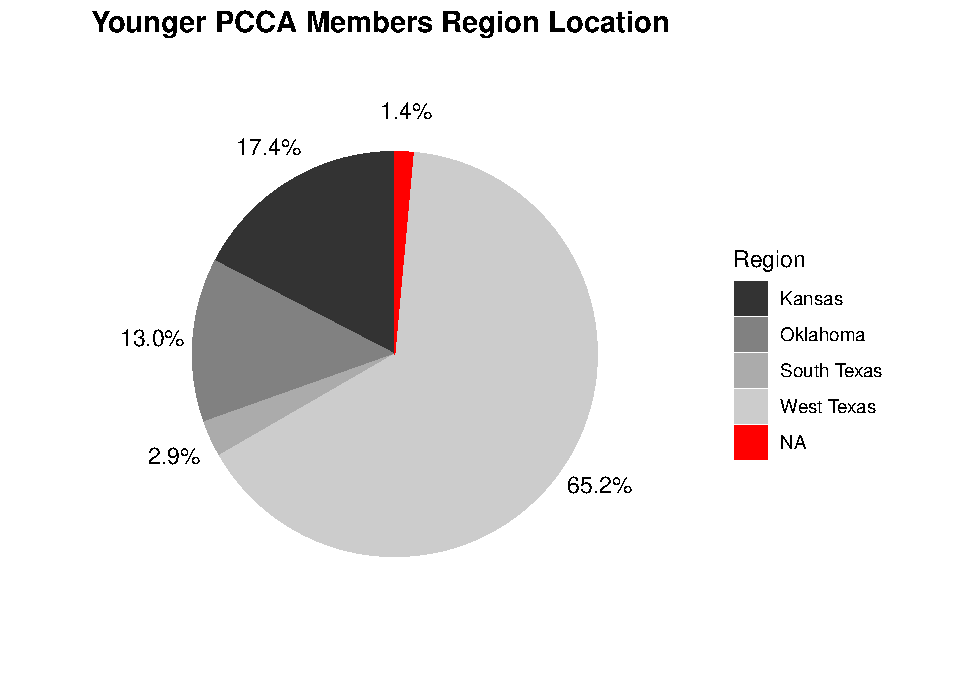
\includegraphics{pcca_survey_files/figure-latex/region-young-1.pdf}

\begin{Shaded}
\begin{Highlighting}[]
\NormalTok{region }\OtherTok{\textless{}{-}}\NormalTok{ older }\SpecialCharTok{\%\textgreater{}\%}
    \FunctionTok{group\_by}\NormalTok{(region) }\SpecialCharTok{\%\textgreater{}\%}
    \FunctionTok{summarise}\NormalTok{(}\AttributeTok{count =} \FunctionTok{n\_distinct}\NormalTok{(number))}

\NormalTok{bp }\OtherTok{\textless{}{-}} \FunctionTok{ggplot}\NormalTok{(region, }\FunctionTok{aes}\NormalTok{(}\AttributeTok{x =} \StringTok{""}\NormalTok{, }\AttributeTok{y =}\NormalTok{ count, }\AttributeTok{fill =}\NormalTok{ region)) }\SpecialCharTok{+}
    \FunctionTok{geom\_bar}\NormalTok{(}\AttributeTok{width =} \DecValTok{1}\NormalTok{, }\AttributeTok{stat =} \StringTok{"identity"}\NormalTok{)}
\NormalTok{pie }\OtherTok{\textless{}{-}}\NormalTok{ bp }\SpecialCharTok{+} \FunctionTok{coord\_polar}\NormalTok{(}\StringTok{"y"}\NormalTok{, }\AttributeTok{start =} \DecValTok{0}\NormalTok{)}

\NormalTok{total }\OtherTok{\textless{}{-}} \FunctionTok{as.numeric}\NormalTok{(}\FunctionTok{nrow}\NormalTok{(older))}

\NormalTok{pie }\SpecialCharTok{+} \FunctionTok{scale\_fill\_grey}\NormalTok{() }\SpecialCharTok{+} \FunctionTok{ggtitle}\NormalTok{(}\StringTok{"Older PCCA Members Region Location"}\NormalTok{) }\SpecialCharTok{+}
\NormalTok{    blank\_theme }\SpecialCharTok{+} \FunctionTok{theme}\NormalTok{(}\AttributeTok{axis.text.x =} \FunctionTok{element\_blank}\NormalTok{()) }\SpecialCharTok{+} \FunctionTok{geom\_text}\NormalTok{(}\FunctionTok{aes}\NormalTok{(}\AttributeTok{x =} \FloatTok{1.7}\NormalTok{,}
    \AttributeTok{label =} \FunctionTok{percent}\NormalTok{(count}\SpecialCharTok{/}\NormalTok{total, }\AttributeTok{accuracy =} \FloatTok{0.1}\NormalTok{)), }\AttributeTok{position =} \FunctionTok{position\_stack}\NormalTok{(}\AttributeTok{vjust =} \FloatTok{0.5}\NormalTok{)) }\SpecialCharTok{+}
    \FunctionTok{guides}\NormalTok{(}\AttributeTok{fill =} \FunctionTok{guide\_legend}\NormalTok{(}\AttributeTok{title =} \StringTok{"Region"}\NormalTok{))}
\end{Highlighting}
\end{Shaded}

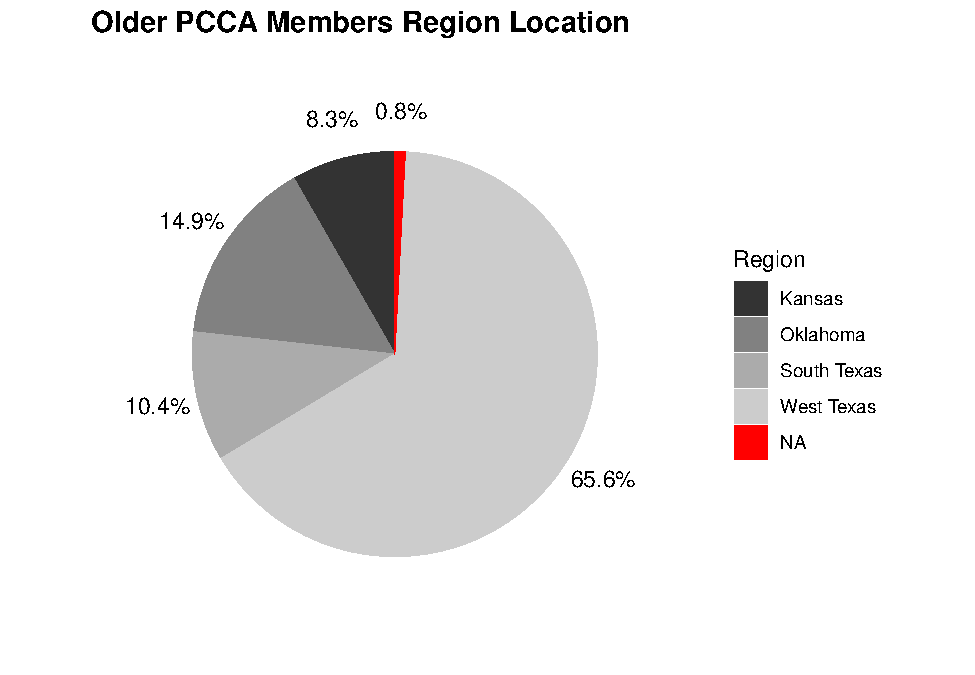
\includegraphics{pcca_survey_files/figure-latex/region-old-1.pdf}

\begin{Shaded}
\begin{Highlighting}[]
\NormalTok{information }\OtherTok{\textless{}{-}}\NormalTok{ younger }\SpecialCharTok{\%\textgreater{}\%}
    \FunctionTok{group\_by}\NormalTok{(}\StringTok{\textasciigrave{}}\AttributeTok{gathering information}\StringTok{\textasciigrave{}}\NormalTok{) }\SpecialCharTok{\%\textgreater{}\%}
    \FunctionTok{summarise}\NormalTok{(}\AttributeTok{count =} \FunctionTok{n\_distinct}\NormalTok{(number))}

\NormalTok{information }\OtherTok{\textless{}{-}}\NormalTok{ information }\SpecialCharTok{\%\textgreater{}\%}
    \FunctionTok{filter}\NormalTok{(information}\SpecialCharTok{$}\NormalTok{count }\SpecialCharTok{\textgreater{}} \DecValTok{4}\NormalTok{)}

\NormalTok{total }\OtherTok{\textless{}{-}} \FunctionTok{as.numeric}\NormalTok{(}\FunctionTok{nrow}\NormalTok{(younger))}

\NormalTok{bp }\OtherTok{\textless{}{-}} \FunctionTok{ggplot}\NormalTok{(information, }\FunctionTok{aes}\NormalTok{(}\AttributeTok{x =} \StringTok{""}\NormalTok{, }\AttributeTok{y =}\NormalTok{ count, }\AttributeTok{fill =} \StringTok{\textasciigrave{}}\AttributeTok{gathering information}\StringTok{\textasciigrave{}}\NormalTok{)) }\SpecialCharTok{+}
    \FunctionTok{geom\_bar}\NormalTok{(}\AttributeTok{width =} \DecValTok{1}\NormalTok{, }\AttributeTok{stat =} \StringTok{"identity"}\NormalTok{)}
\NormalTok{pie }\OtherTok{\textless{}{-}}\NormalTok{ bp }\SpecialCharTok{+} \FunctionTok{coord\_polar}\NormalTok{(}\StringTok{"y"}\NormalTok{, }\AttributeTok{start =} \DecValTok{0}\NormalTok{)}

\NormalTok{pie }\SpecialCharTok{+} \FunctionTok{scale\_fill\_grey}\NormalTok{() }\SpecialCharTok{+} \FunctionTok{ggtitle}\NormalTok{(}\StringTok{"Younger PCCA Members Preferred Information Sources"}\NormalTok{) }\SpecialCharTok{+}
\NormalTok{    blank\_theme }\SpecialCharTok{+} \FunctionTok{theme}\NormalTok{(}\AttributeTok{axis.text.x =} \FunctionTok{element\_blank}\NormalTok{()) }\SpecialCharTok{+} \FunctionTok{geom\_text}\NormalTok{(}\FunctionTok{aes}\NormalTok{(}\AttributeTok{x =} \FloatTok{1.7}\NormalTok{,}
    \AttributeTok{label =} \FunctionTok{percent}\NormalTok{(count}\SpecialCharTok{/}\NormalTok{total, }\AttributeTok{accuracy =} \FloatTok{0.1}\NormalTok{)), }\AttributeTok{position =} \FunctionTok{position\_stack}\NormalTok{(}\AttributeTok{vjust =} \FloatTok{0.5}\NormalTok{)) }\SpecialCharTok{+}
    \FunctionTok{guides}\NormalTok{(}\AttributeTok{fill =} \FunctionTok{guide\_legend}\NormalTok{(}\AttributeTok{title =} \StringTok{"Types of sources"}\NormalTok{))}
\end{Highlighting}
\end{Shaded}

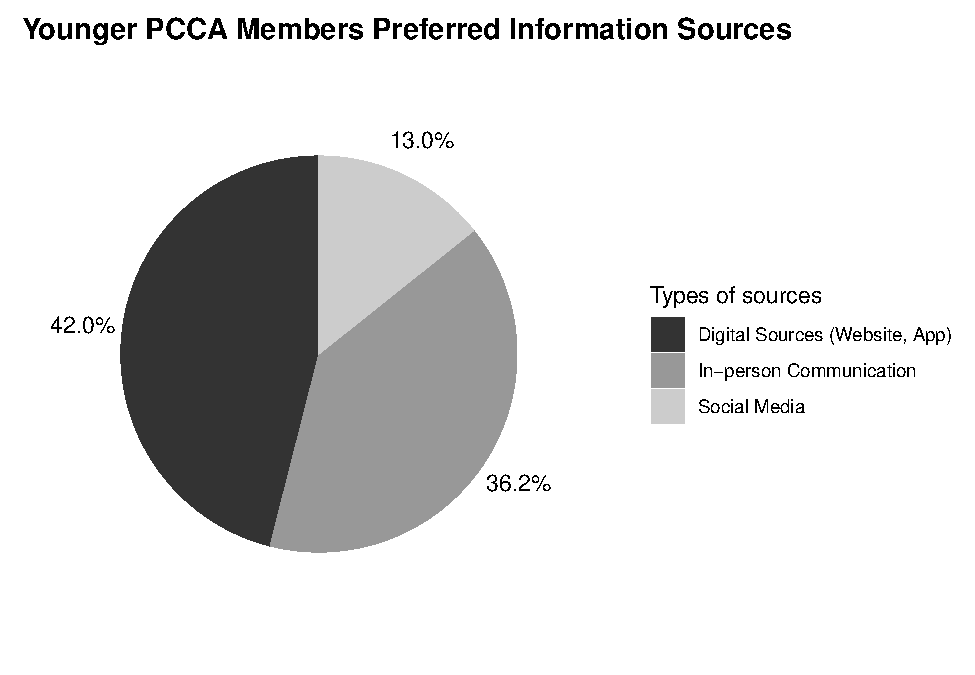
\includegraphics{pcca_survey_files/figure-latex/information-young-1.pdf}

\begin{Shaded}
\begin{Highlighting}[]
\NormalTok{information }\OtherTok{\textless{}{-}}\NormalTok{ older }\SpecialCharTok{\%\textgreater{}\%}
    \FunctionTok{group\_by}\NormalTok{(}\StringTok{\textasciigrave{}}\AttributeTok{gathering information}\StringTok{\textasciigrave{}}\NormalTok{) }\SpecialCharTok{\%\textgreater{}\%}
    \FunctionTok{summarise}\NormalTok{(}\AttributeTok{count =} \FunctionTok{n\_distinct}\NormalTok{(number))}

\NormalTok{information }\OtherTok{\textless{}{-}}\NormalTok{ information }\SpecialCharTok{\%\textgreater{}\%}
    \FunctionTok{filter}\NormalTok{(information}\SpecialCharTok{$}\NormalTok{count }\SpecialCharTok{\textgreater{}} \DecValTok{4}\NormalTok{)}

\NormalTok{total }\OtherTok{\textless{}{-}} \FunctionTok{as.numeric}\NormalTok{(}\FunctionTok{nrow}\NormalTok{(older))}

\NormalTok{bp }\OtherTok{\textless{}{-}} \FunctionTok{ggplot}\NormalTok{(information, }\FunctionTok{aes}\NormalTok{(}\AttributeTok{x =} \StringTok{""}\NormalTok{, }\AttributeTok{y =}\NormalTok{ count, }\AttributeTok{fill =} \StringTok{\textasciigrave{}}\AttributeTok{gathering information}\StringTok{\textasciigrave{}}\NormalTok{)) }\SpecialCharTok{+}
    \FunctionTok{geom\_bar}\NormalTok{(}\AttributeTok{width =} \DecValTok{1}\NormalTok{, }\AttributeTok{stat =} \StringTok{"identity"}\NormalTok{)}
\NormalTok{pie }\OtherTok{\textless{}{-}}\NormalTok{ bp }\SpecialCharTok{+} \FunctionTok{coord\_polar}\NormalTok{(}\StringTok{"y"}\NormalTok{, }\AttributeTok{start =} \DecValTok{0}\NormalTok{)}

\NormalTok{pie }\SpecialCharTok{+} \FunctionTok{scale\_fill\_grey}\NormalTok{() }\SpecialCharTok{+} \FunctionTok{ggtitle}\NormalTok{(}\StringTok{"Older PCCA Members Preferred Information Sources"}\NormalTok{) }\SpecialCharTok{+}
\NormalTok{    blank\_theme }\SpecialCharTok{+} \FunctionTok{theme}\NormalTok{(}\AttributeTok{axis.text.x =} \FunctionTok{element\_blank}\NormalTok{()) }\SpecialCharTok{+} \FunctionTok{geom\_text}\NormalTok{(}\FunctionTok{aes}\NormalTok{(}\AttributeTok{x =} \FloatTok{1.7}\NormalTok{,}
    \AttributeTok{label =} \FunctionTok{percent}\NormalTok{(count}\SpecialCharTok{/}\NormalTok{total, }\AttributeTok{accuracy =} \FloatTok{0.1}\NormalTok{)), }\AttributeTok{position =} \FunctionTok{position\_stack}\NormalTok{(}\AttributeTok{vjust =} \FloatTok{0.5}\NormalTok{)) }\SpecialCharTok{+}
    \FunctionTok{guides}\NormalTok{(}\AttributeTok{fill =} \FunctionTok{guide\_legend}\NormalTok{(}\AttributeTok{title =} \StringTok{"Types of sources"}\NormalTok{))}
\end{Highlighting}
\end{Shaded}

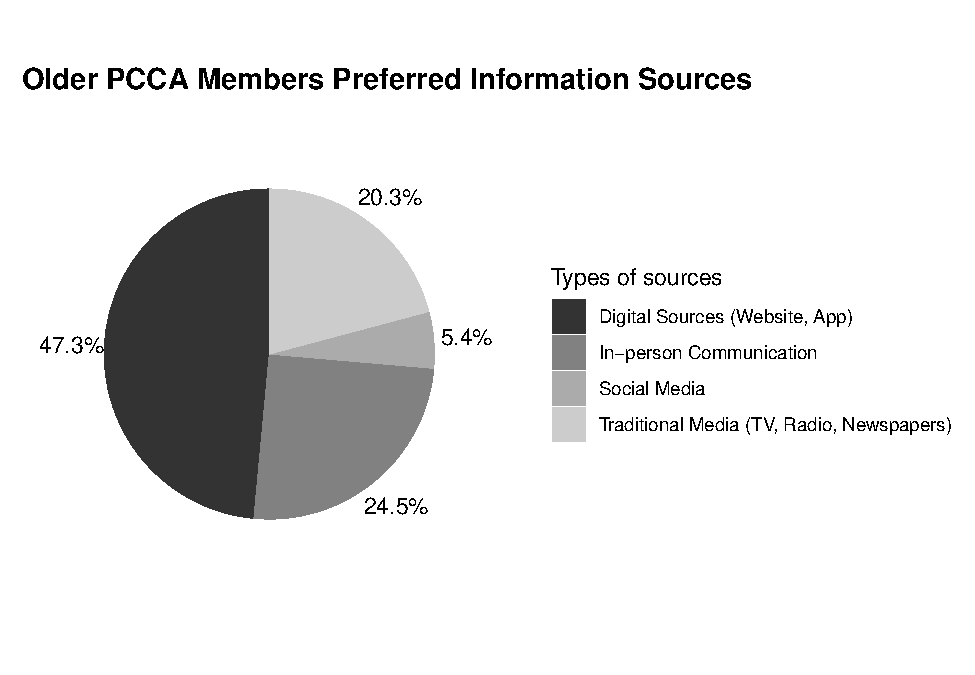
\includegraphics{pcca_survey_files/figure-latex/information-old-1.pdf}

\begin{Shaded}
\begin{Highlighting}[]
\NormalTok{marketing }\OtherTok{\textless{}{-}}\NormalTok{ younger }\SpecialCharTok{\%\textgreater{}\%}
    \FunctionTok{group\_by}\NormalTok{(}\StringTok{\textasciigrave{}}\AttributeTok{most used marketing method}\StringTok{\textasciigrave{}}\NormalTok{) }\SpecialCharTok{\%\textgreater{}\%}
    \FunctionTok{summarise}\NormalTok{(}\AttributeTok{count =} \FunctionTok{n\_distinct}\NormalTok{(number))}

\NormalTok{lbls }\OtherTok{\textless{}{-}} \FunctionTok{paste}\NormalTok{(}\FunctionTok{names}\NormalTok{(marketing), }\StringTok{"}\SpecialCharTok{\textbackslash{}n}\StringTok{"}\NormalTok{, marketing, }\AttributeTok{sep =} \StringTok{""}\NormalTok{)}

\NormalTok{total }\OtherTok{\textless{}{-}} \FunctionTok{as.numeric}\NormalTok{(}\FunctionTok{nrow}\NormalTok{(younger))}

\NormalTok{bp }\OtherTok{\textless{}{-}} \FunctionTok{ggplot}\NormalTok{(marketing, }\FunctionTok{aes}\NormalTok{(}\AttributeTok{x =} \StringTok{""}\NormalTok{, }\AttributeTok{y =}\NormalTok{ count, }\AttributeTok{fill =} \StringTok{\textasciigrave{}}\AttributeTok{most used marketing method}\StringTok{\textasciigrave{}}\NormalTok{)) }\SpecialCharTok{+}
    \FunctionTok{geom\_bar}\NormalTok{(}\AttributeTok{width =} \DecValTok{1}\NormalTok{, }\AttributeTok{stat =} \StringTok{"identity"}\NormalTok{)}
\NormalTok{pie }\OtherTok{\textless{}{-}}\NormalTok{ bp }\SpecialCharTok{+} \FunctionTok{coord\_polar}\NormalTok{(}\StringTok{"y"}\NormalTok{, }\AttributeTok{start =} \DecValTok{0}\NormalTok{)}

\NormalTok{pie }\SpecialCharTok{+} \FunctionTok{ggtitle}\NormalTok{(}\StringTok{"Most Used Marketing Method"}\NormalTok{) }\SpecialCharTok{+}\NormalTok{ blank\_theme }\SpecialCharTok{+} \FunctionTok{theme}\NormalTok{(}\AttributeTok{axis.text.x =} \FunctionTok{element\_blank}\NormalTok{()) }\SpecialCharTok{+}
    \FunctionTok{geom\_text}\NormalTok{(}\FunctionTok{aes}\NormalTok{(}\AttributeTok{x =} \FloatTok{1.7}\NormalTok{, }\AttributeTok{label =} \FunctionTok{percent}\NormalTok{(count}\SpecialCharTok{/}\NormalTok{total, }\AttributeTok{accuracy =} \FloatTok{0.1}\NormalTok{)),}
        \AttributeTok{position =} \FunctionTok{position\_stack}\NormalTok{(}\AttributeTok{vjust =} \FloatTok{0.5}\NormalTok{)) }\SpecialCharTok{+} \FunctionTok{guides}\NormalTok{(}\AttributeTok{fill =} \FunctionTok{guide\_legend}\NormalTok{(}\AttributeTok{title =} \StringTok{"Marketing methods"}\NormalTok{))}
\end{Highlighting}
\end{Shaded}

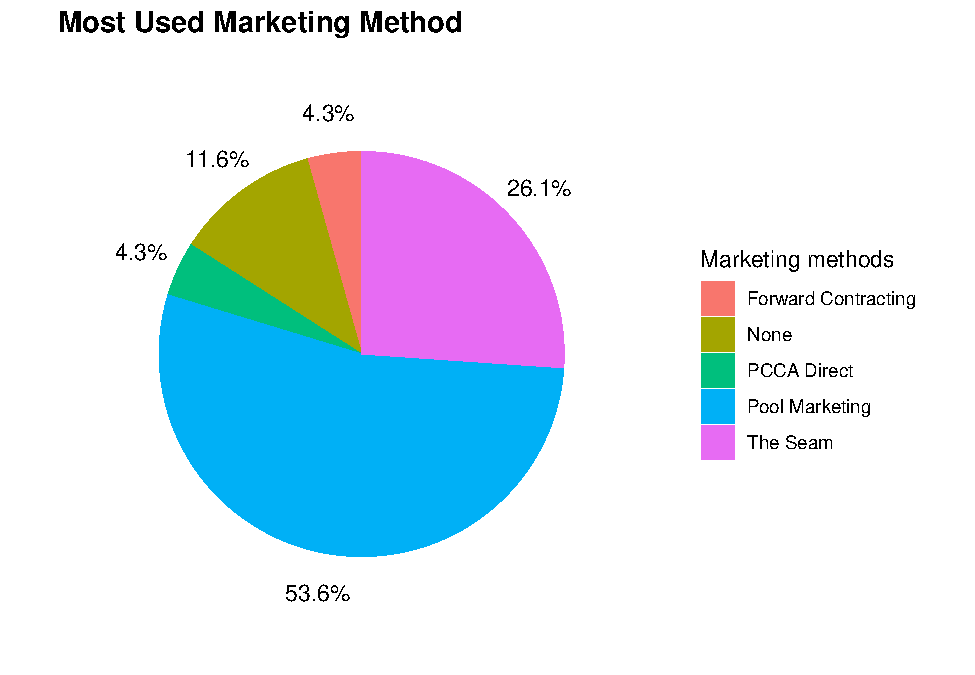
\includegraphics{pcca_survey_files/figure-latex/marketing-young-1.pdf}

\begin{Shaded}
\begin{Highlighting}[]
\NormalTok{marketing }\OtherTok{\textless{}{-}}\NormalTok{ older }\SpecialCharTok{\%\textgreater{}\%}
    \FunctionTok{group\_by}\NormalTok{(}\StringTok{\textasciigrave{}}\AttributeTok{most used marketing method}\StringTok{\textasciigrave{}}\NormalTok{) }\SpecialCharTok{\%\textgreater{}\%}
    \FunctionTok{summarise}\NormalTok{(}\AttributeTok{count =} \FunctionTok{n\_distinct}\NormalTok{(number))}

\NormalTok{lbls }\OtherTok{\textless{}{-}} \FunctionTok{paste}\NormalTok{(}\FunctionTok{names}\NormalTok{(marketing), }\StringTok{"}\SpecialCharTok{\textbackslash{}n}\StringTok{"}\NormalTok{, marketing, }\AttributeTok{sep =} \StringTok{""}\NormalTok{)}

\NormalTok{total }\OtherTok{\textless{}{-}} \FunctionTok{as.numeric}\NormalTok{(}\FunctionTok{nrow}\NormalTok{(older))}

\NormalTok{bp }\OtherTok{\textless{}{-}} \FunctionTok{ggplot}\NormalTok{(marketing, }\FunctionTok{aes}\NormalTok{(}\AttributeTok{x =} \StringTok{""}\NormalTok{, }\AttributeTok{y =}\NormalTok{ count, }\AttributeTok{fill =} \StringTok{\textasciigrave{}}\AttributeTok{most used marketing method}\StringTok{\textasciigrave{}}\NormalTok{)) }\SpecialCharTok{+}
    \FunctionTok{geom\_bar}\NormalTok{(}\AttributeTok{width =} \DecValTok{1}\NormalTok{, }\AttributeTok{stat =} \StringTok{"identity"}\NormalTok{)}
\NormalTok{pie }\OtherTok{\textless{}{-}}\NormalTok{ bp }\SpecialCharTok{+} \FunctionTok{coord\_polar}\NormalTok{(}\StringTok{"y"}\NormalTok{, }\AttributeTok{start =} \DecValTok{0}\NormalTok{)}

\NormalTok{pie }\SpecialCharTok{+} \FunctionTok{ggtitle}\NormalTok{(}\StringTok{"Most Used Marketing Method"}\NormalTok{) }\SpecialCharTok{+}\NormalTok{ blank\_theme }\SpecialCharTok{+} \FunctionTok{theme}\NormalTok{(}\AttributeTok{axis.text.x =} \FunctionTok{element\_blank}\NormalTok{()) }\SpecialCharTok{+}
    \FunctionTok{geom\_text}\NormalTok{(}\FunctionTok{aes}\NormalTok{(}\AttributeTok{x =} \FloatTok{1.7}\NormalTok{, }\AttributeTok{label =} \FunctionTok{percent}\NormalTok{(count}\SpecialCharTok{/}\NormalTok{total, }\AttributeTok{accuracy =} \FloatTok{0.1}\NormalTok{)),}
        \AttributeTok{position =} \FunctionTok{position\_stack}\NormalTok{(}\AttributeTok{vjust =} \FloatTok{0.5}\NormalTok{)) }\SpecialCharTok{+} \FunctionTok{guides}\NormalTok{(}\AttributeTok{fill =} \FunctionTok{guide\_legend}\NormalTok{(}\AttributeTok{title =} \StringTok{"Marketing methods"}\NormalTok{))}
\end{Highlighting}
\end{Shaded}

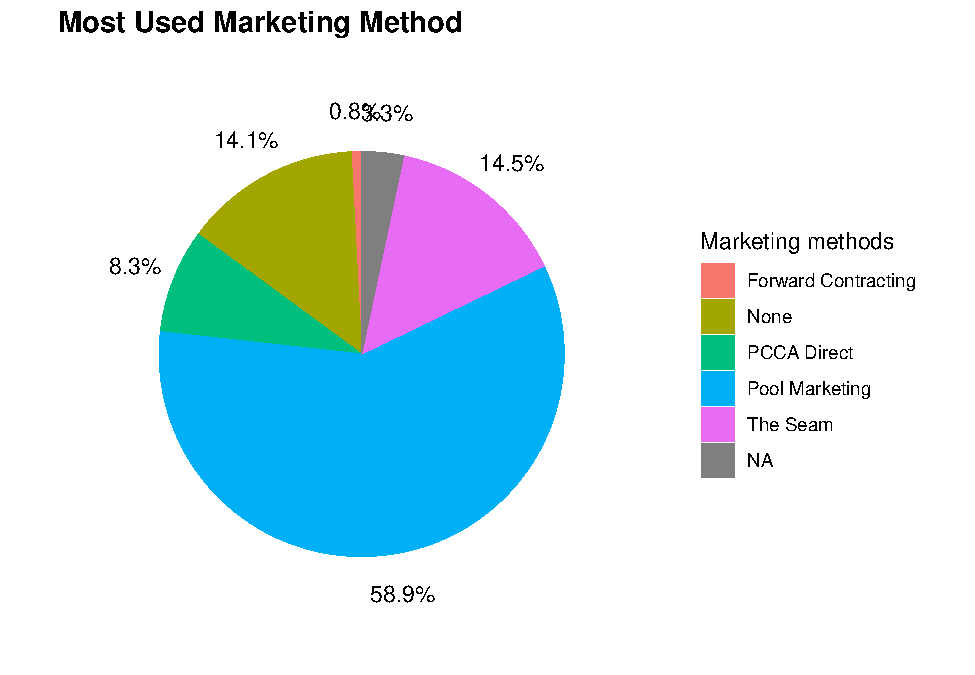
\includegraphics{pcca_survey_files/figure-latex/marketing-old-1.pdf}

\hypertarget{percentages}{%
\section{Percentages}\label{percentages}}

\hypertarget{knowledge}{%
\subsection{Knowledge}\label{knowledge}}

\begin{Shaded}
\begin{Highlighting}[]
\NormalTok{knowledge.cols }\OtherTok{\textless{}{-}} \FunctionTok{c}\NormalTok{(}\StringTok{"number"}\NormalTok{, }\StringTok{"marketing pool"}\NormalTok{, }\StringTok{"the seam"}\NormalTok{, }\StringTok{"pcca direct"}\NormalTok{,}
    \StringTok{"forward contracting"}\NormalTok{, }\StringTok{"gen"}\NormalTok{)}

\NormalTok{knowledge.younger }\OtherTok{\textless{}{-}}\NormalTok{ younger }\SpecialCharTok{\%\textgreater{}\%}
    \FunctionTok{select}\NormalTok{(knowledge.cols)}

\NormalTok{knowledge.older }\OtherTok{\textless{}{-}}\NormalTok{ older }\SpecialCharTok{\%\textgreater{}\%}
    \FunctionTok{select}\NormalTok{(knowledge.cols)}
\end{Highlighting}
\end{Shaded}

\begin{Shaded}
\begin{Highlighting}[]
\NormalTok{knowledge.yo }\OtherTok{\textless{}{-}} \FunctionTok{bind\_rows}\NormalTok{(knowledge.younger, knowledge.older)}
\end{Highlighting}
\end{Shaded}

\begin{Shaded}
\begin{Highlighting}[]
\NormalTok{stat.test }\OtherTok{\textless{}{-}}\NormalTok{ knowledge.yo }\SpecialCharTok{\%\textgreater{}\%}
    \FunctionTok{t\_test}\NormalTok{(}\StringTok{\textasciigrave{}}\AttributeTok{forward contracting}\StringTok{\textasciigrave{}} \SpecialCharTok{\textasciitilde{}}\NormalTok{ gen) }\SpecialCharTok{\%\textgreater{}\%}
    \FunctionTok{add\_significance}\NormalTok{()}

\NormalTok{stat.test}
\end{Highlighting}
\end{Shaded}

\begin{verbatim}
## # A tibble: 1 x 9
##   .y.                 group1 group2    n1    n2 statistic    df       p p.signif
##   <chr>               <chr>  <chr>  <int> <int>     <dbl> <dbl>   <dbl> <chr>   
## 1 forward contracting older  young~   241    69     -2.63  120. 0.00967 **
\end{verbatim}

\end{document}
